\documentclass[utf8x,notes,pagenumber,hyperref={pagebackref=true,citecolor=green,bookmarks=true,pdfpagelabels=true}]{beamer} %remove draft when done with tex prep
%\documentclass[notes]{beamer} 
\usepackage{etex}
\usepackage{beamerthemesplit}
\usetheme{PaloAlto} %Hannover, Belin, Warsaw, PaloAlto, Frankfurt, Berkeley  etc

% Itemize breaks compilation: https://tex.stackexchange.com/questions/414419/put-bullets-in-a-block-inside-itemize-environment
\usefonttheme{professionalfonts}
\setbeamertemplate{itemize items}[ball]
\setbeamercolor{block title}{fg=white, bg=blue!70!black}
\setbeamercolor{block body}{fg=black, bg=gray!20}
\setbeamertemplate{blocks}[rounded][shadow=true]

\usepackage{pgfpages}
\usepackage{xcolor}
\definecolor{light-blue}{rgb}{0.95,0.55,.9}
\definecolor{light-red}{rgb}{0.95,0.15,.19}
\mode<handout>{\setbeamercolor{background canvas sidebar}{bg=red!45}}
\setbeamercolor{structure}{fg=light-blue}
\usepackage{bm}
\usepackage{subfloat}
\usepackage{paralist}
\usepackage{subcaption}
\usepackage{amssymb, amsmath}
\usepackage{mathrsfs}
\usepackage[round]{natbib}
\usepackage{algorithm}
\usepackage{algpseudocode}
\bibliographystyle{unsrtnat}
\usepackage[export]{adjustbox}
\usepackage{array,booktabs,tabularx}
\usepackage{tikz}
\usetikzlibrary{shapes,arrows, circuits, patterns, snakes, decorations.pathreplacing}
\usepackage{schemabloc, verbatim}
\usepackage{graphicx}

\usepackage{media9} % for video embeddings
\usepackage{multimedia} % for video embeddings
\usepackage{tcolorbox}
\tcbuselibrary{theorems}
\newcommand{\tcb}[2]
{
 \begin{tcolorbox}[title=\text{#2}]
 #1
 \end{tcolorbox}
}

%\renewcommand\thefootnote{}\footnote{#1}
\definecolor{light-blue}{rgb}{0.30,0.35,1}
\definecolor{light-green}{rgb}{0.20,0.49,.85}
\definecolor{purple}{rgb}{0.70,0.69,.2}

\newcommand{\lb}[1]{\textcolor{light-blue}{#1}}
\newcommand{\bl}[1]{\textcolor{blue}{#1}}

\newcommand{\maybe}[1]{\textcolor{gray}{\textbf{MAYBE: }{#1}}}
\newcommand{\inspect}[1]{\textcolor{cyan}{\textbf{CHECK THIS: }{#1}}}
\newcommand{\more}[1]{\textcolor{red}{\textbf{MORE: }{#1}}}

% FYA
\newcommand{\cmt}[1]{{\footnotesize\textcolor{red}{#1}}}%{#2}
%\newcommand{\note}[1]{\cmt{Note: #1}}
%\newcommand{\todo}[1]{\textcolor{cyan}{TO-DO: #1}}
\newcommand{\review}[1]{\noindent\textcolor{red}{$\rightarrow$ #1}}
\newcommand{\response}[1]{\noindent{#1}}
\newcommand{\stopped}[1]{\color{red}STOPPED HERE #1\hrulefill}

%Text commands
\newcounter{mnote}
\newcommand{\marginote}[1]{\addtocounter{mnote}{1}\marginpar{\themnote. \scriptsize #1}}
\setcounter{mnote}{0}
% \newcommand{\comment}[1]{}
\newcommand{\ie}{$i.e.$\ }
\newcommand{\eg}{e.g.\ }
\newcommand{\cf}{c.f.\ }
\newcommand{\yes}{\checkmark}
\newcommand{\no}{\ding{55}}

%Reference commands
\newcommand{\flabel}[1]{\label{fig:#1}}
\newcommand{\seclabel}[1]{\label{sec:#1}}
\newcommand{\tlabel}[1]{\label{tab:#1}}
\newcommand{\elabel}[1]{\label{eq:#1}}
\newcommand{\alabel}[1]{\label{alg:#1}}
\newcommand{\fref}[1]{\cref{fig:#1}}
\newcommand{\sref}[1]{\cref{sec:#1}}
\newcommand{\tref}[1]{\cref{tab:#1}}
\newcommand{\eref}[1]{\cref{eq:#1}}
\newcommand{\aref}[1]{\cref{alg:#1}}

\newcommand{\bull}[1]{$\bullet$ #1}
\newcommand{\argmax}{\text{argmax}}
\newcommand{\argmin}{\text{argmin}}
\newcommand{\mc}[1]{\mathcal{#1}}
\newcommand{\bb}[1]{\mathbb{#1}}


\def\tidx{t}
%\def\comment
%\def\value{V}
% from https://www.cs.jhu.edu/~jason/advice/write-the-paper-first.html
\newcommand{\Note}[1]{}
\renewcommand{\Note}[1]{\hl{[#1]}}  % comment out this definition to suppress all Notes
%\algnewcommand\algorithmicforeach{\textbf{for each}}
%\algdef{S}[FOR]{Foreach}[1]{\algorithmicforeach\ #1\ \algorithmicdo} %

%\newcolumntype{M}[1]{>{\centering\arraybackslash}m{#1}}
\def\coriolis{\textbf{\textit{C}}}
\def\massinertia{\textbf{\textit{M}}}
\def\torque{\bm{\tau}}
\def\frictionvec{\textbf{\textit{f}}}
\def\Smat{\textbf{\textit{S}}}
\def\Bmat{\textbf{\textit{B}}}
\def\wheelrad{\textbf{\textit{r}}}

\def\stateweight{\textbf{\textit{w}}_x}
\def\actionweight{\textbf{\textit{w}}_u}
\def\advactionweight{\textbf{\textit{w}}_v}

%Thesis defs
%\def\upchi{\textchi}
\def\kau{\mc{K}}
\def\particle{\bm{x}}
\def\deformationgrad{\textbf{F}}
\def\refconf{\bm{\upchi}_0}
\def\refconfbody{\mathscr{B}_0}
\def\conf{\bm{\upchi}}
\def\currconf{\bm{\upchi}}
\def\Eulerian{\mc{E}}
\def\cauchystress{\bm{\sigma}}
\def\stresscomp{\sigma}
\def\currconfbody{\mathscr{B}}
\def\materialresponse{\textbf{G}}
\def\orthoggroup{{\textit{SO}}(3)}
\def\liegroup{{\textit{SE}}(3)}
\def\liealgebra{\mathfrak{se}(3)}
\def\identity{\textbf{I}}
\newcommand{\trace}[1]{\textbf{tr}(#1)}
\def\leftcauchy{\textbf{B}}
\def\rightcauchy{\textbf{C}}
\def\fiber{\textbf{dx}}

\def\dof{\text{DOF }}
\def\dofs{\text{DOFs }}
\def\reline{\mathbb{R}}
\def\curve{\deformationgrad}
\def\twist{{\xi}}
\def\contactforce{\tilde{F}}
\def\contactforcecomp{f}
\def\gaussianmap{\textbf{}n}
\def\contacttorquecomp{\tau}
\def\wrt{with respect to }
\def\curveparam{\position}
\def\basis{\bm{e}}
\def\pose{{g}}
\def\selmap{{B}}
\def\manipmap{{G}}
\def\jacob{\bm{J}}
\def\normal{\bm{n}}
\def\position{\textbf{r}}
\def\deformationgradcur{\textbf{H}}
\def\eulerianvel{\textbf{v}(\position, t)}
\def\headparam{\zeta}
\def\strain{\mathrm{\Psi}}
\def\strainiso{\mathrm{\Psi_{\text{iso}}}}
\def\strainfiber{\mathrm{\Psi_{\text{mesh}}}}

% mechanism defs
\def\wallthickness{1cm}
\def\sorodiam{9 cm}
\def\sorodiamdim{5-6.25cm}

% inline macros
\newcommand{\putsoro}[2]{\includegraphics[width=.45\columnwidth,height=#2\columnwidth]{../../../PhDThesis/figures/#1}}
\newcommand{\sorowidth}{.35}


%\newtheorem{theorem}{Theorem}[]
%\newtheorem{example}{Example}
%\newtheorem{homework}{Homework}

\tikzstyle{block} = [draw, fill=yellow!80, rectangle,minimum height=3em, minimum width=4em]
\tikzstyle{sum} = [draw, fill=white!20, circle, node distance=1cm]
\tikzstyle{input} = [coordinate]
\tikzstyle{output} = [coordinate]
\tikzstyle{pinstyle} = [pin edge={to-,thin,black}]

\newcolumntype{Z}{>{\centering\arraybackslash}X} % centered tabularx columns
\newcommand{\pphantom}{\textcolor{ta3aluminium}} % phantom
%\setbeamerfont{title}{shape=\itshape,family=\rmfamily}
\setbeamercolor{title}{fg=magenta!70!black,bg=yellow!70!white}
%
\title{\small A short treatise on robots' geometry, kinematics, and dynamics.}

\author{Author: Lekan Molu}
\institute{
	%
	\vspace{0.5em}
	%
	Dissemination Venue: Microsoft Research RL Group, \\
	New York City, NY 10012 
}

%\date{\today} 
\date{June 09, 2022} 


\setbeamersize{sidebar width left=2cm}
%remove title and author names from sidebar
  \makeatletter
\setbeamertemplate{sidebar \beamer@sidebarside}%{sidebar theme}
{
	\beamer@tempdim=\beamer@sidebarwidth%
	\advance\beamer@tempdim by -6pt%
	\insertverticalnavigation{\beamer@sidebarwidth}%
	\vfill
	\ifx\beamer@sidebarside\beamer@lefttext%
	\else%
	\usebeamercolor{normal text}%
	\llap{\usebeamertemplate***{navigation symbols}\hskip0.1cm}%
	\vskip2pt%
	\fi%
}%
\makeatother

\begin{document}
	\maketitle
%http://tug.ctan.org/macros/latex/contrib/beamer/doc/beameruserguide.pdf#subsection.21.3
\begin{frame}
	\frametitle{Table of Contents}
	\tableofcontents
\end{frame}

\lecture{Robot Mechanisms}{Mechanisms and Pairs}
\chapter{Preamble}
\label{chap:intro}

Consider this your roadmap for the course.  Please read through the syllabus posted on moodle carefully and feel free to share any questions that you may have.  Please print a copy of the syllabus for reference. Some relevant parts of the syllabus are repeated here but the moodle reference should serve as your guide throughout the ten weeks of this course.

\section{Course Description}
This course focuses on the algorithmic and mathematical concepts  with respect to robot planning, manipulation and control. Topics covered include kinematics and dynamics, as well as path planning and deep reinforcement learning algorithms. Simulations and experiments on hardware testbeds (listed in the syllabus) will be performed to test the related algorithms.

\section{Course Outcomes}
After taking this course, each student will be able to

\begin{itemize}
\item Develop planning and manipulation schemes to drive robot operation

\item Integrate perception algorithms into manipulation and planning systems

\item Determine the kinematic description of a robot's motion or locomotion
\end{itemize}

\section{Prerequisites}

RBOT 210 or an advanced knowledge of ROS; undergraduate-level experience or equivalent with object oriented programming; strong programming knowledge in Python and C++ is required; and RBOT 205 if mathematical foundational skills of admissions criteria are needed.

\section{Recommended Texts}
\begin{itemize}
	\item  	Main Texts
	\begin{itemize}
		\item Murray, R. M., Li, Z., and Sastry, S. S. (1994). A Mathematical Introduction to Robotic Manipulation. Book (Vol. 29). Free PDF preprint downloadable from, \href{https://www.cds.caltech.edu/~murray/books/MLS/pdf/mls94-complete.pdf }{Murray's website}.
		%
		\item 	Spong, M. W., Hutchinson, S., and Vidyasagar, M. (2012). Robot Modeling and Control. Students can buy from this \href{https://www.amazon.com/Robot-Modeling-Control-Mark-Spong/dp/0471649902}{Amazon Link}.
	\end{itemize} 
	%
	\item Secondary Text
	%
	\begin{itemize}
		\item Modern Robotics: Mechanics, Planning, and Control. Free PDF preprint downloadable from \href{ http://hades.mech.northwestern.edu/images/7/7f/MR.pdf}{Author's Northwestern Website}.		
	\end{itemize} 
    %
    \item 
    Auxiliary Text: 
    %
    \begin{itemize}
    	\item Theory of Screws: A Study in the Dynamics of a Rigid Body by Robert Stawell Ball, Dublin: Hodges, Foster, and Co., Grafton-Street (Should be downloadable via Interlibrary Loan).
    \end{itemize}
\end{itemize}

\section{Recommended Journals}
	%
	\begin{itemize}
		\item 
		\href{ https://ieeexplore.ieee.org/xpl/RecentIssue.jsp?punumber=8860}{IEEE Transactions on Robotics}.
		%
		\item 
		\href{https://journals.sagepub.com/home/ijr}{The International Journal of Robotics Research}.
		%
		\item 
		\href{https://www.ieee-ras.org/conferences-workshops/fully-sponsored/icra}{The IEEE International Conference on Robotics and Automation}.
		%
		\item \href{https://www.ieee-ras.org/conferences-workshops/financially-co-sponsored/iros}{IEEE/Robotics Society of Japan International Conference on Intelligent Robots and Systems (IROS)}.
		%
		\item \href{https://www.journals.elsevier.com/robotics-and-autonomous-systems}{Robotics and Autonomous Systems, An Elsevier Journal}.
	\end{itemize}

\section{Required Software}
	
	\begin{itemize}
	%
	\item A working knowledge of python and the anaconda environment.
	%
	\item \href{https://www.ros.org/}{The Robot Operating System}.
	%
	\item ROS from Conda installation \href{ https://medium.com/@wolfv/ros-on-conda-forge-dca6827ac4b6}{instructions}.
	\end{itemize}

\section{Online Course Content}
%
This course will be conducted completely online using Brandeis’ LATTE \href{http://moodle2.brandeis.edu}{site}. The site contains the course syllabus, assignments, our discussion forums, links/resources to course-related professional organizations and sites, and weekly checklists, objectives, outcomes, topic notes, self-tests, and discussion questions.  Access information is emailed to enrolled participants before the start of the course.   To begin participating in the course, review the ``Welcoming Message" and the ``Week 1 Checklist."

\section{Assessments and Labs}

Please read the syllabus posted on the RBOT 250 website thoroughly.

\section{Errata}

If in the course of using these notes, you find sentence errors, errata or mistakes in equations, please annotate them and upload it to the discussion forum. Points will awarded, at the discretion of the instructor, for such help.
\section{Pairs, Linkages, and Configurations}

\begin{frame}
	\frametitle{Lecture One Outline}
	\begin{tcolorbox}[coltitle=white!80,colframe=blue!85,split=.2,title=Mechanism Components]
		Kinematic geometry. Mechanisms.
		\tcblower
		Joints: Joint closure; Pairs; Couplings.
		\vspace{.2cm}
		\newline
		Lower pairs and linkages; Higher and lower pairs.
		\vspace{.2cm}
		\newline
		Motions: Planar and spherical motions.
		\vspace{.2cm}
		\newline
		Synthesis: Type-, number-, and size-syntheses.
	\end{tcolorbox}
\end{frame}

\subsection{Mechanics}
\begin{frame}
	\frametitle{Preamble.}
	%
	\begin{block}{Mechanics}
		\textcolor{blue}{Mechanics} is an indirect study of nature via \textcolor{red}{bodies} --  essentially the mathematical abstractions of common natural things; the \textcolor{red}{mass} is an \textcolor{blue}{\textit{allocation}} in \textcolor{blue}{\textit{place}} to each body.
	\end{block}

	\begin{block}{Geometry}
		 \textcolor{red}{Geometry}, deals with the \textcolor{red}{theory of places}; geometry is the bedrock of \textcolor{red}{robotics, control theory}, and many fields of \textcolor{red}{modern engineering and the physical sciences}.
\end{block}
\end{frame}

\begin{frame}
	\frametitle{Mechanics Overview.}
	%
	\begin{definition}[Motion]
		When a  \textcolor{blue}{place} undergoes \textcolor{red}{body transformation} in the course of  \textcolor{red}{time}, we have \textcolor{red}{motion}.
	\end{definition}
\end{frame}

\begin{frame}
	\frametitle{Preamble -- Mass, Body, Rigid Body Motion.}
	%		
	\begin{definition}[Body -- Truesdell, 1977.]
		By a \textcolor{blue}{body}, we shall mean the \textcolor{red}{closure of an open set} in some \textcolor{red}{measure space} $\Omega$ over which a \textcolor{red}{non-negative measure $M$, called the mass}, is defined, and that $M$ can be extended to a Borel measure over the $\sigma-$ algebra of Borel sets in $\Omega$.
	\end{definition}
\end{frame}

\begin{frame}
	\frametitle{Preamble -- Mass, Body, Rigid Body Motion.}
	%	
	\begin{block}{Bodies -- Truesdell, 1977.}
		That in \textcolor{blue}{mechanics} which deals with  \begin{inparaenum}[(i)]
			\item \textcolor{red}{mass points}, which occupy a single point at any one time;
			\item \textcolor{red}{rigid bodies}, which never deform;
			\item \textcolor{red}{strings and rods and jets}, which are 1-dimensional;  membranes and shells, that sweep out surfaces;
			\item \textcolor{red}{space-filling fluids and solids} e.t.c.
		\end{inparaenum}   
		\textcolor{blue}{are termed bodies}.
	\end{block}
\end{frame}


\begin{frame}
	\frametitle{Statics, Dynamics, Rigid Body (Motion).}
	%		
	\begin{block}{Statics and Dynamics}
		That which studies \textcolor{blue}{putative equilibria} is referred to as  \textcolor{red}{statics}. That which concerns  \textcolor{blue}{motion of all sorts} is referred to as  \textcolor{red}{dynamics}. The dynamics that are specific to  \textcolor{red}{particular bodies} are termed  \textcolor{red}{constitutive}.
	\end{block}
\end{frame}


\begin{frame}
	\frametitle{Statics, Dynamics, Rigid Body (Motion).}
	%	
	\begin{block}{The Rigid Body}
		A \textcolor{blue}{rigid body} does not \textcolor{red}{stretch, buckle, contract, bend, twist, nor deform}. Well, not really!
	\end{block}
	%
	\begin{block}{The Rigid Body}
		As engineers and roboticists, we judge  \textcolor{blue}{kinematic rigid hardware} with the expectation that kinematic changes do not depart from rigid-body predictions.
	\end{block}
	%
\end{frame}

\begin{frame}
	\frametitle{Statics, Dynamics, Rigid Body (Motion).}
	%
	\begin{block}{The Rigid Body}
		We expect that \textcolor{light-blue}{localized stresses}, \textcolor{red}{active noise},  \textcolor{cyan}{vibrations} and \textcolor{magenta}{heat} e.t.c will not cause \textcolor{light-red}{reasonable departures} from expectations.
	\end{block}
	%	
	\begin{block}{Rigid Body Motion}
		That \textcolor{blue}{motion} that \textcolor{red}{preserves distance} between all points in a body is termed a \textcolor{red}{rigid body motion}.
	\end{block}
	%
\end{frame}

\begin{frame}
	\frametitle{Statics, Dynamics, Rigid Body (Motion).}
	%		
	\begin{block}{Rigid Body Motion}
		At issue are components of a rigid body's \textcolor{red}{movement} w.r.t to a fixed or moving \textcolor{blue}{frame of reference}. In its most basic form, this movement is parameterized by \textcolor{red}{displacement} (and is sometimes time-varying e.g. for a continuum body). When solving for the movements of bodies, it is often useful to include velocities (\textcolor{red}{twists}) in order to characterize the \textcolor{red}{motion}.
	\end{block}
\end{frame}


\begin{frame}
	\frametitle{Kinematics vs. Kinetics}
	\begin{block}{Dynamics}
		\begin{align}
			\dot{x} &= f(t; x, u),  \quad x(t_0) = t_0 \\
			\dot{x} &= f(t; x)  + g(t; x, u),  \quad x(t_0) = t_0 
		\end{align}
	\end{block}
	%
	\begin{definition}[Kinematics.] \textcolor{blue}{{Kinematics}} is the English version of the word  \textcolor{blue}{\textit{cin{\'e}matique}} coined by A.M. Amp{\`e}re (1775-1836), who translated it from the Greek word \textcolor{red}{\textit{k{\'i}$\nu \eta \mu \alpha$}}.
	\end{definition}
\end{frame}

\begin{frame}
	\frametitle{Kinematics vs. Kinetics.}
	\begin{definition}[Truesdell]
		That part of a system's \textcolor{blue}{dynamics} that involves its \textcolor{red}{motion} by \textcolor{cyan}{displacement} -- both linear and angular -- and \textcolor{red}{separated from motions owing to forces and  torques}, together with the successive derivatives with respect to time of all such displacements (this includes \textcolor{brown}{velocities, accelerations, and hyper accelerations}) all form the \textcolor{red}{kinematics} of a \textcolor{light-blue}{{rigid}}, \textcolor{light-blue}{{continuum}} or \textcolor{light-blue}{{laminae}} of bodies.
	\end{definition}
\end{frame}


\begin{frame}
	\frametitle{Kinematics vs. Kinetics}
	%
	\begin{block}{Kinetics}
		The \textcolor{blue}{motion} of bodies can also be conceived as resulting from the  \textcolor{red}{forces' action}.  \textcolor{red}{Energy, temperature, and calory} of a body are resultant effects of gains or loss of heat. Motions arising as a result of these are called \textcolor{blue}{kinetics}.
	\end{block}
\end{frame}


\begin{frame}
	\frametitle{Kinematics vs. Kinetics.}
	\begin{definition}[Kinetics -- Technical Definition]
		That part of a system's \textcolor{blue}{dynamics} that involves its \textcolor{red}{motion} by \textcolor{cyan}{forces, energy, torque, inertia, dynamic stability, and equilibrium} and similar properties all form the \textcolor{red}{kinetics} of a \textcolor{light-blue}{{rigid}}, \textcolor{light-blue}{{continuum}} or \textcolor{light-blue}{{laminae}} of bodies.
	\end{definition}
\end{frame}

\begin{frame}
	\frametitle{Kinematic Geometry.}
	\begin{definition}[Kinematic Geometry]
		The \textcolor{blue}{solid geometry of relatively moving rigid bodies} is termed the \textcolor{red}{kinematic geometry} of the rigid body. With \textcolor{light-blue}{motion}, we'd have to include the \textcolor{gray}{successive derivatives of the displacement such as acceleration} e.t.c as the `laws of motion' stipulates in mechanics.
	\end{definition}
\end{frame}



\begin{frame}
	\frametitle{Joints and Links}
	%
	\begin{block}{Links}
		\textcolor{light-blue}{Links} may be \textcolor{brown}{rigid mechanical parts, elastic, (vulcanized) rubber components, diaphragms, conveyor belts, spring-damper systems} e.t.c.
	\end{block}
	%
	\begin{block}{An Elementary Joint or Kinematic Pair.}
		An \textcolor{magenta}{elementary joint} or a \textcolor{light-blue}{kinematic pair} consists of touching two \textcolor{red}{links} \textcolor{light-blue}{together at one point} -- then ensuring a single contact point is \textcolor{purple}{continuously maintained} throughout \textcolor{light-blue}{relative movement}. 
	\end{block}
\end{frame}



\begin{frame}
	\frametitle{Joint (Contact) Kinematics}
	%
	\begin{block}{Contact Kinematics}
		A body may \textcolor{red}{slide} or  \textcolor{purple}{slip} across a \textcolor{light-blue}{plane or surface}, or \textcolor{green}{roll} over another body. 
	\end{block}
	%
	\begin{block}{Joints}
		\textcolor{blue}{Joints} are the result of the \textcolor{red}{connecting points} between two or more \textcolor{pink}{rigid bodies}.
	\end{block}
	%
\end{frame}

\subsection{Mechanisms}
\begin{frame}
	\frametitle{Definition of a Mechanism}
	\begin{definition}[Author's Definition]
		A \textcolor{blue}{connection} of  \textcolor{cyan}{mechanical, magnetic, electrical, hydraulic, or pneumatic components} forming an \textcolor{magenta}{assemblage}, meant for moving \textcolor{pink}{rigid, semi-rigid or non-rigid bodies} via a \textcolor{green}{controlled generation} of (sometimes constrained) \textcolor{red}{motion}.
	\end{definition}
	%
	\begin{tcolorbox}[coltitle=red!80!black,colframe=magenta!25,title=Kenneth Hunt (1978)]
		A means of \textcolor{green}{transmitting}, \textcolor{gray}{controlling}, or \textcolor{red}{constraining} the relative movement between parts. Whenever we have an \textcolor{blue}{higher pair} or more, we have a mechanism. 
	\end{tcolorbox}
\end{frame}


\begin{frame}
	\frametitle{Mechanism Examples}
	\begin{tabular}{|c|c|} 
		%
		\hline  \\
		Spring-Mass-Damper System & Excavator \\
		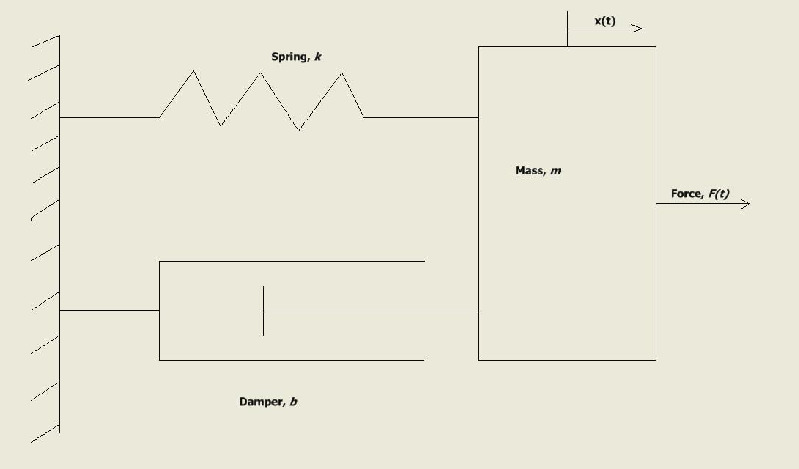
\includegraphics[height=5em,width=10em]{figures/spring-mass-damper.jpg} & 
		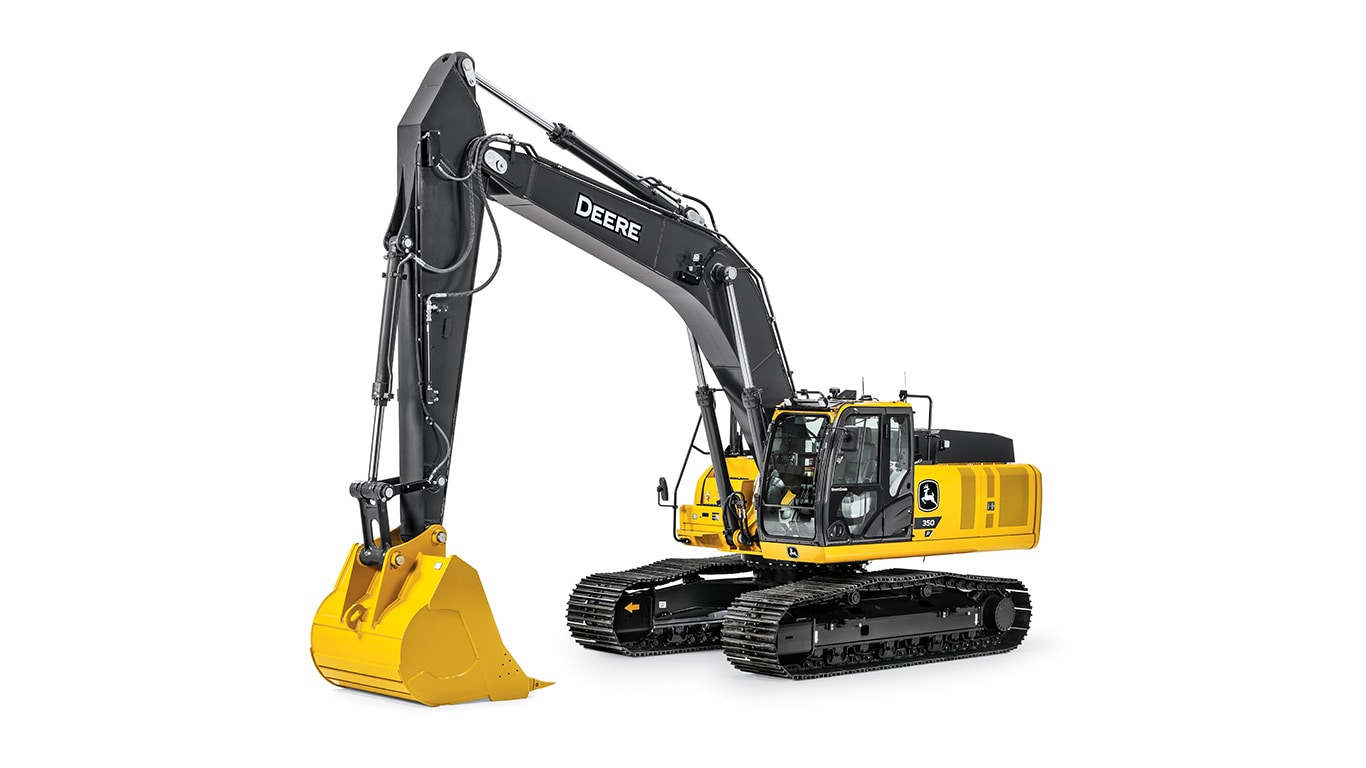
\includegraphics[height=5em,width=10em]{figures/excavJohnDeere.jpg} \\
		\hline \\
		Car suspension & Daimler  Plant \\
		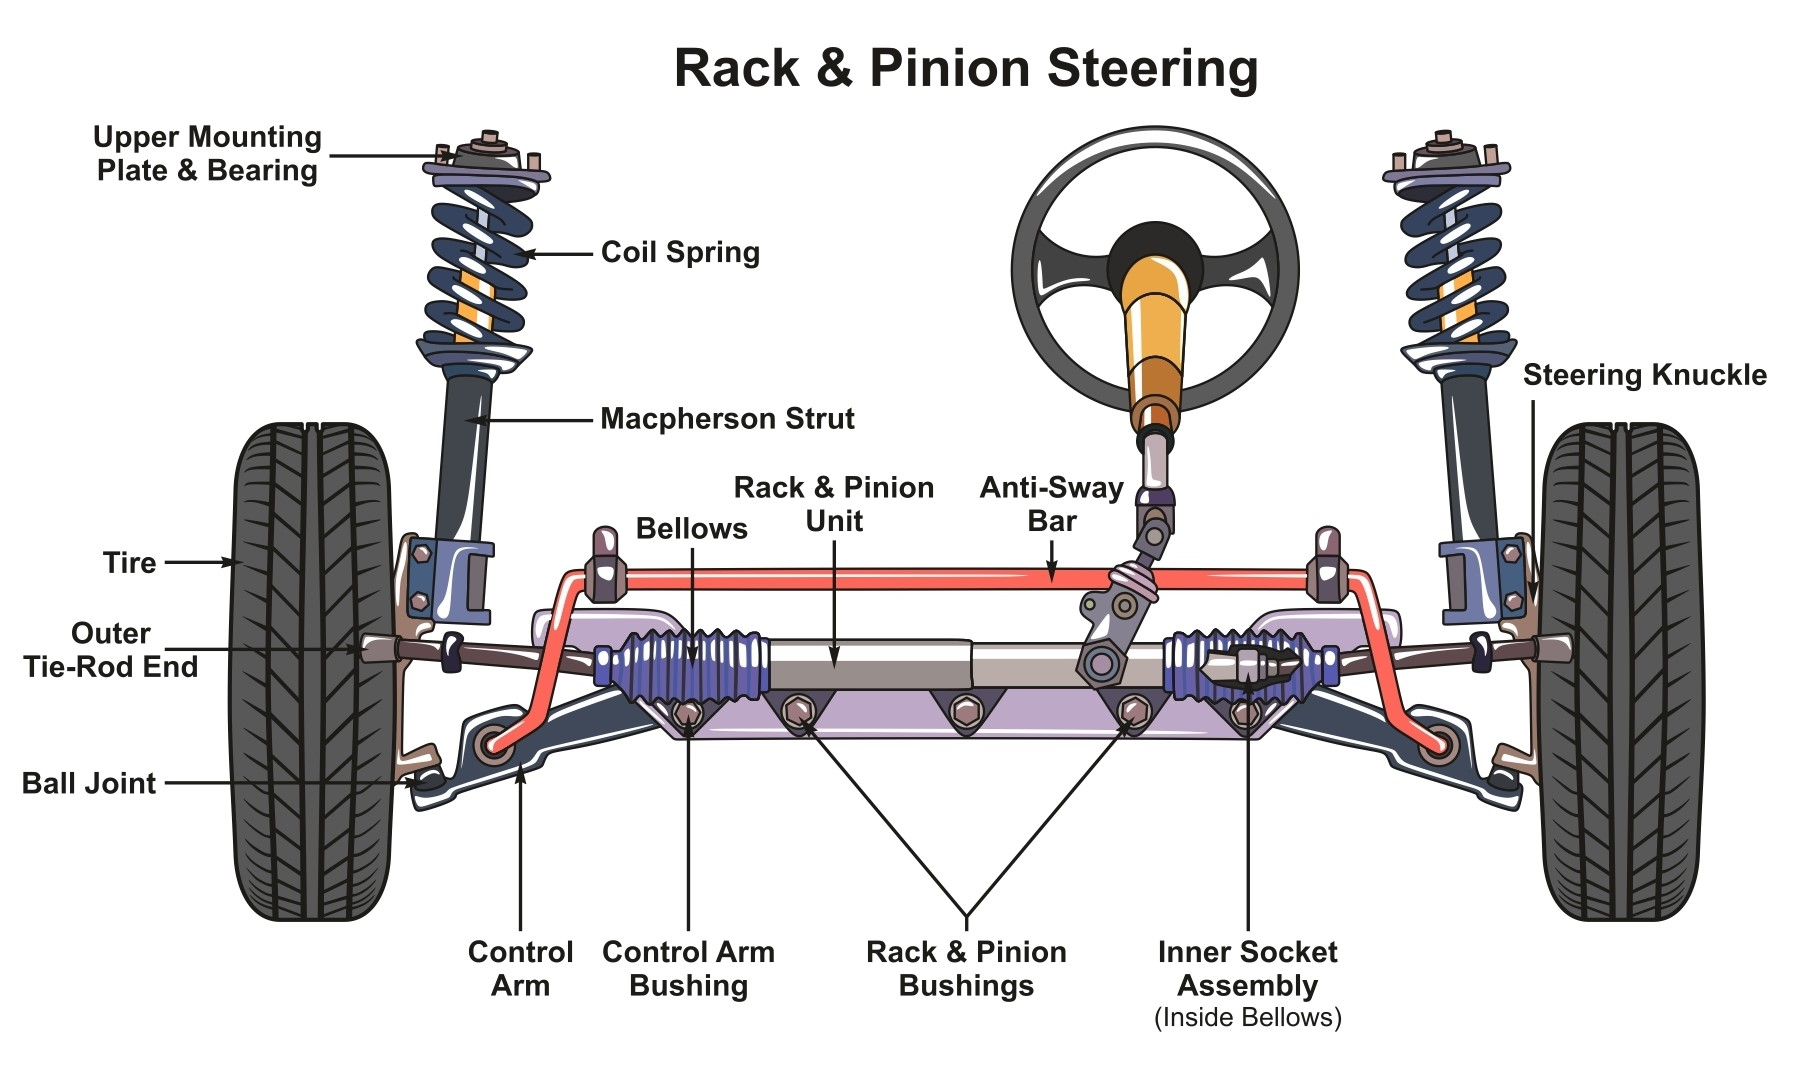
\includegraphics[height=5em,width=10em]{figures/carsusp.jpg} &
		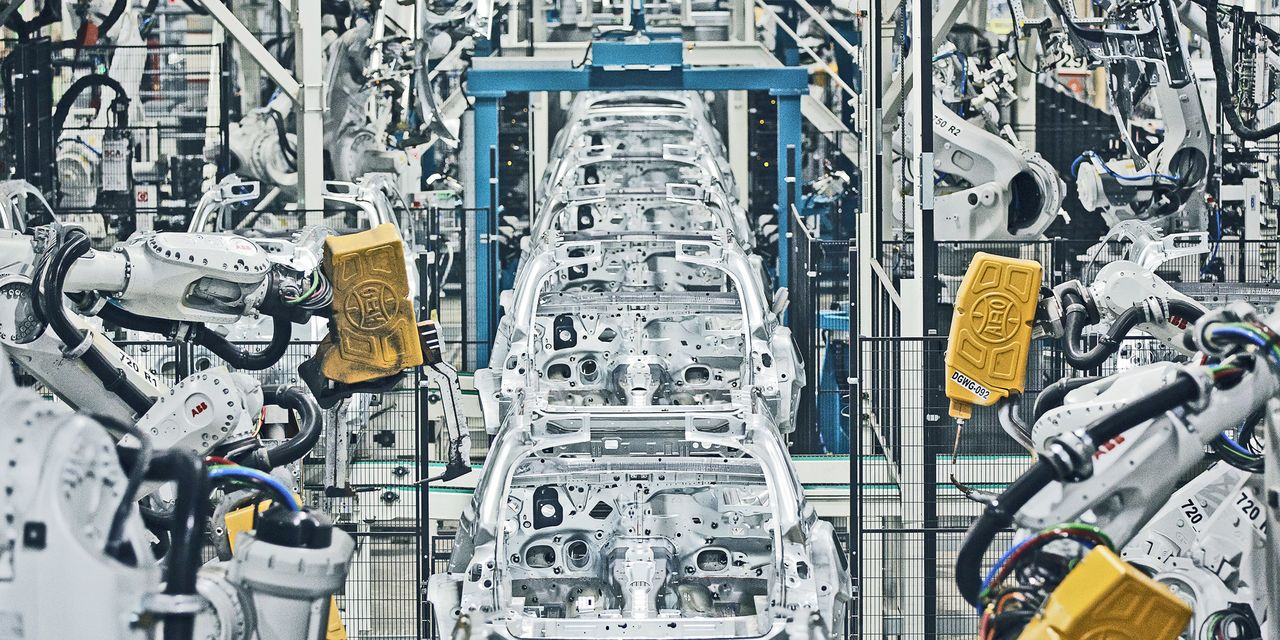
\includegraphics[height=5em,width=10em]{figures/daimler_manuf.jpeg} \\
		\hline
	\end{tabular}
\end{frame}

\subsection{Pairs and Linkages}
\begin{frame}
	\frametitle{Lower Pairs, Higher Pairs, Linkages}
	%
	\begin{block}{Lower and Higher Pairs}
		When elements of pairs touch one another over a \textcolor{red}{substantial region of a surface covering a line, curve-surface, or point of contact}, we have \textcolor{blue}{lower pairs}. When they touch \textcolor{red}{along a discrete line, curve-surface, or point of contact}, we have \textcolor{blue}{higher pairs}.
	\end{block}
	%
	\begin{block}{Linkage (Hunt, 1978)}
		If all joints of a \textcolor{red}{mechanism or mechanical movement} belong to lower pairs, we have a \textcolor{blue}{linkage}. 
	\end{block}
	%
\end{frame}

\begin{frame}
	\frametitle{Prismatic Pairs or $P$-pairs}
	%
	\begin{columns}[t]	
	\begin{column}{.56\textwidth}
		\begin{block}{Hunt, 1978}
		{Formed by receding the axis of the revolution surface between two pairs to $\infty$ so that the \textcolor{blue}{curve} that produces the surface moves parallel to itself, \textcolor{green}{tracing a cylinder}; or a \textcolor{blue}{polygonal-tracing curve} generates a \textcolor{green}{prism}.}
		\end{block}
	\end{column}
		
	\begin{column}{.45\textwidth}
		\begin{figure}
			\centering
			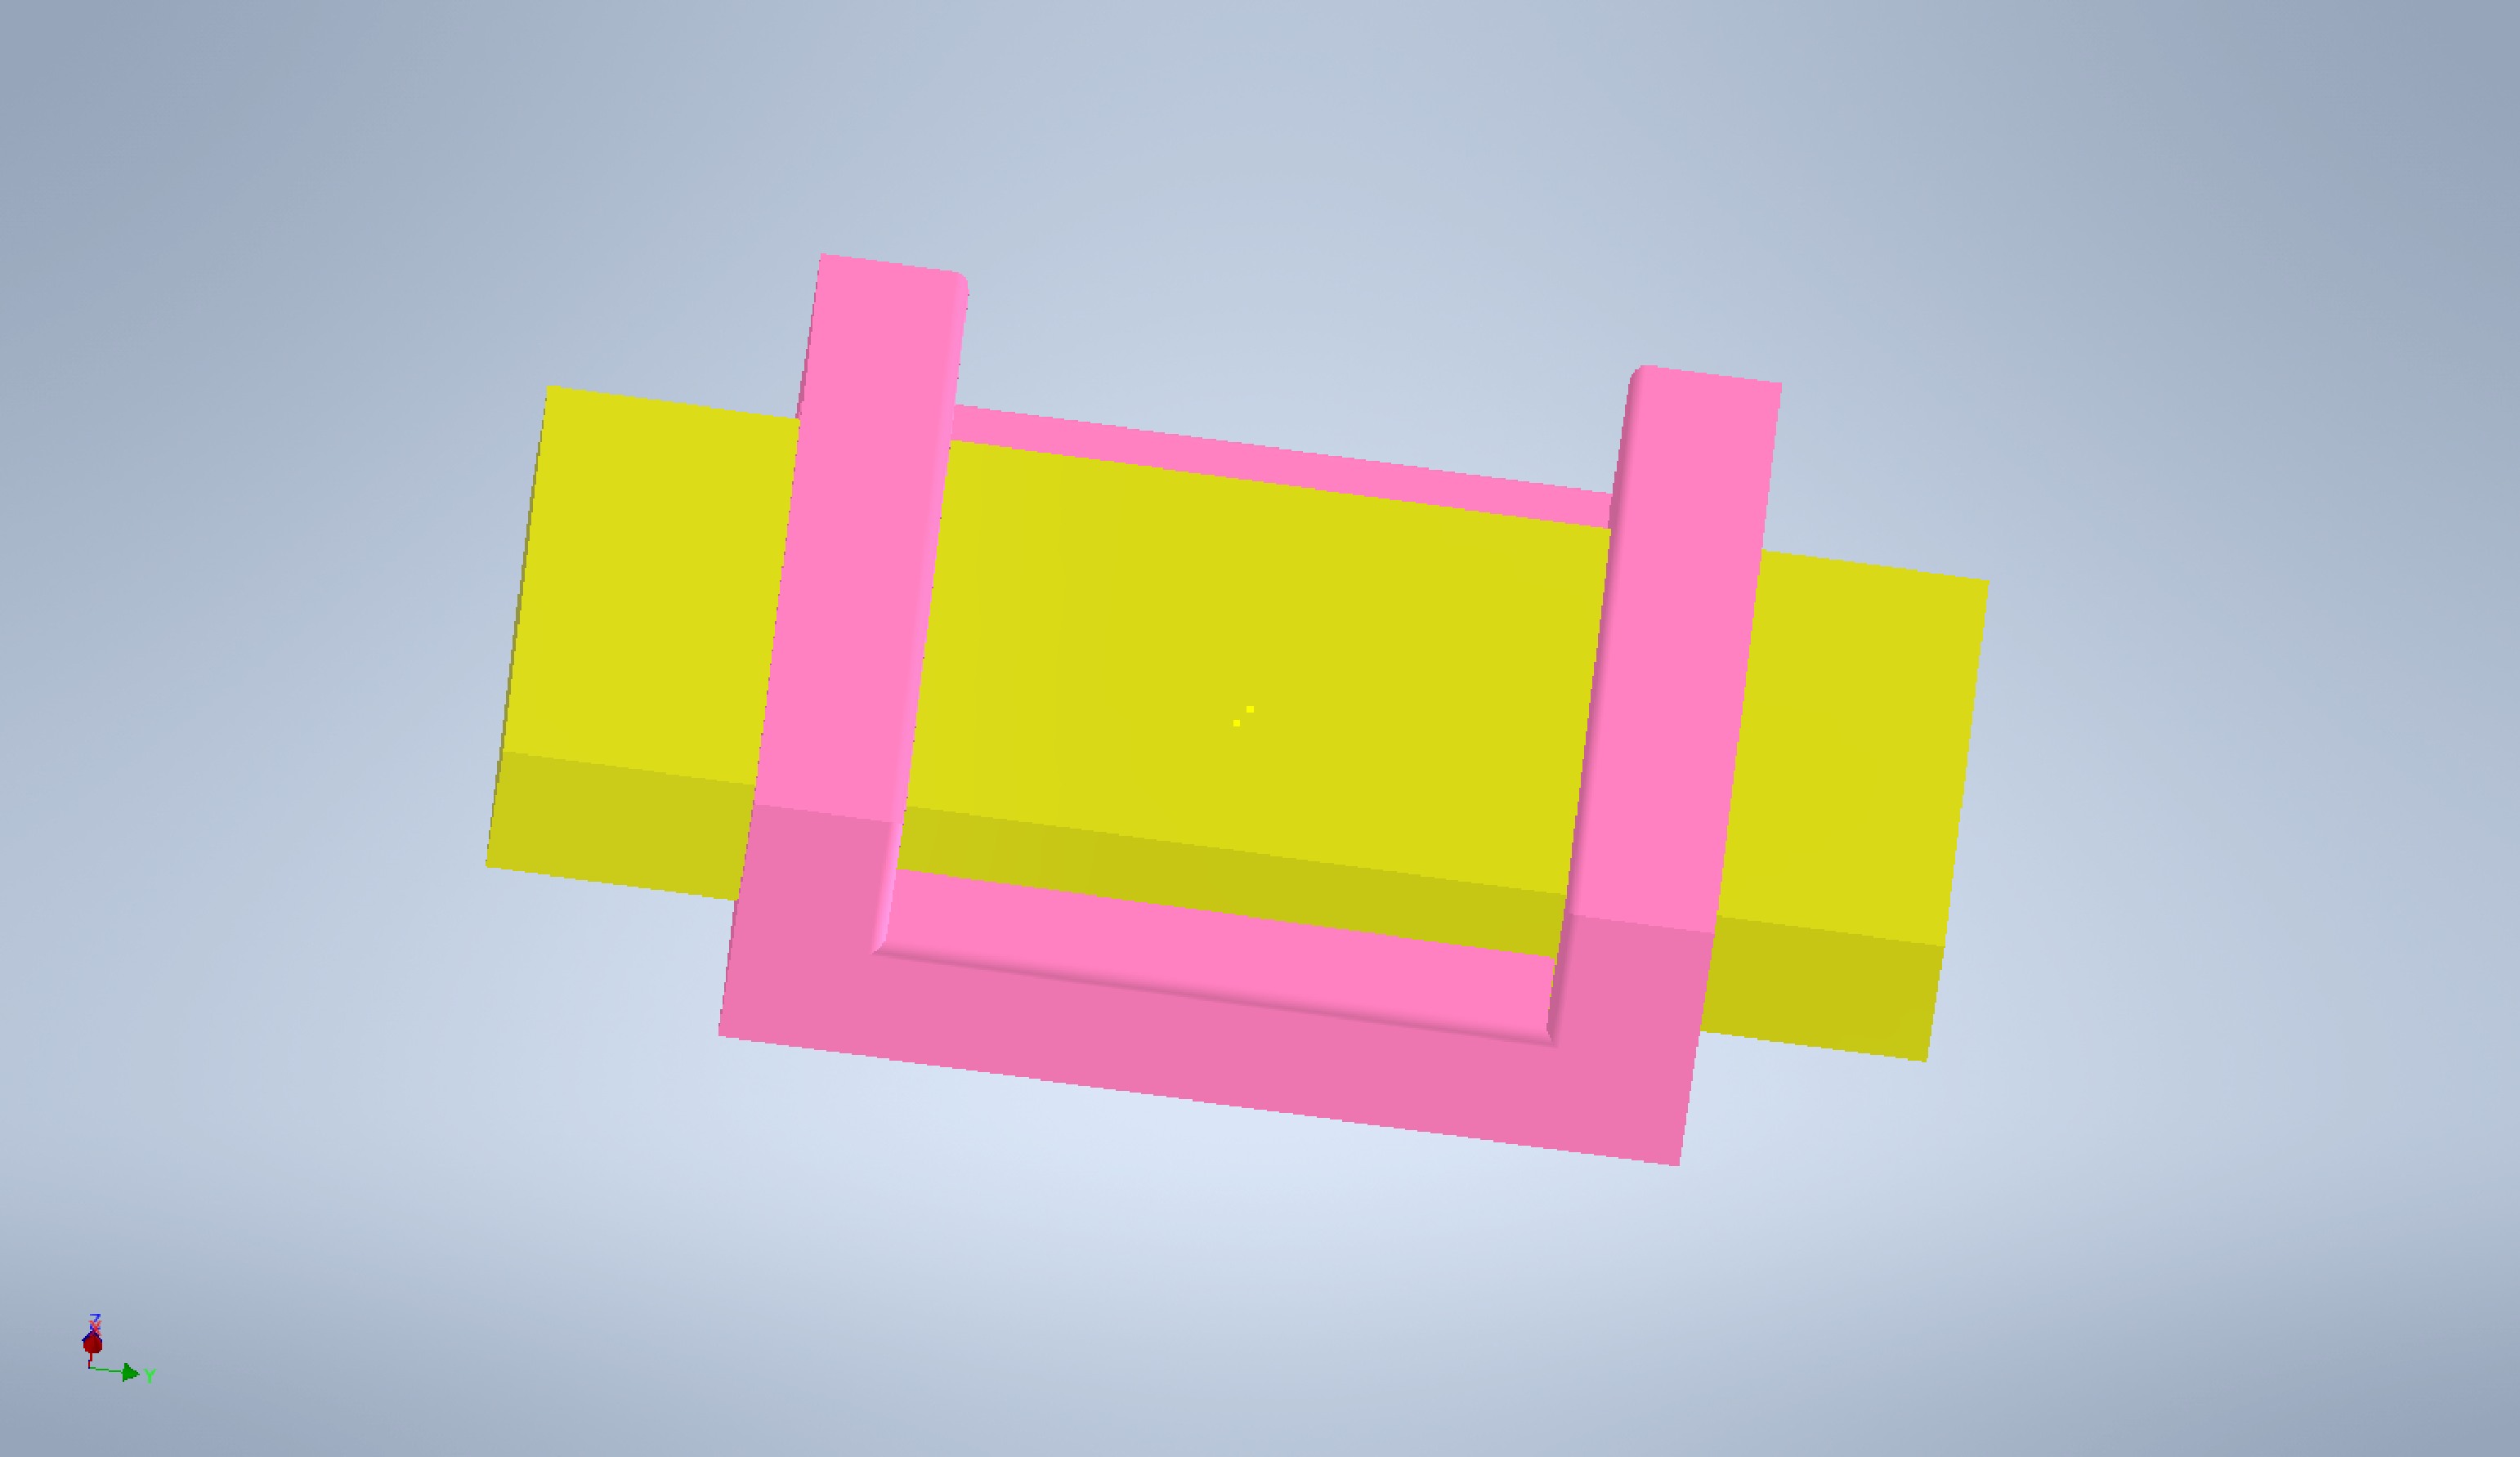
\includegraphics[width=\textwidth]{../Notes/figures/prismatic_joint.pdf}
		\end{figure}
	\end{column}
	\end{columns}
\end{frame}

\begin{frame}
	\frametitle{Revolute Pairs or $R$-pairs}
	%
	\footnotesize{One \textcolor{red}{convex surface} and \textcolor{red}{one non-convex} surface for a \textcolor{green}{one degree of rotational freedom} around the one \textcolor{blue}{joint} the two surfaces make.}
	%\note{An R-pair has a convex and non-convex surface. Revolution surface can be traced by any general curve, outside a planar curve or a circle with axis of revolution about center as it produces an $S$-pair element.}
	\begin{columns}[t]		
		\begin{column}{.5\textwidth}
			\begin{figure}
				\centering
				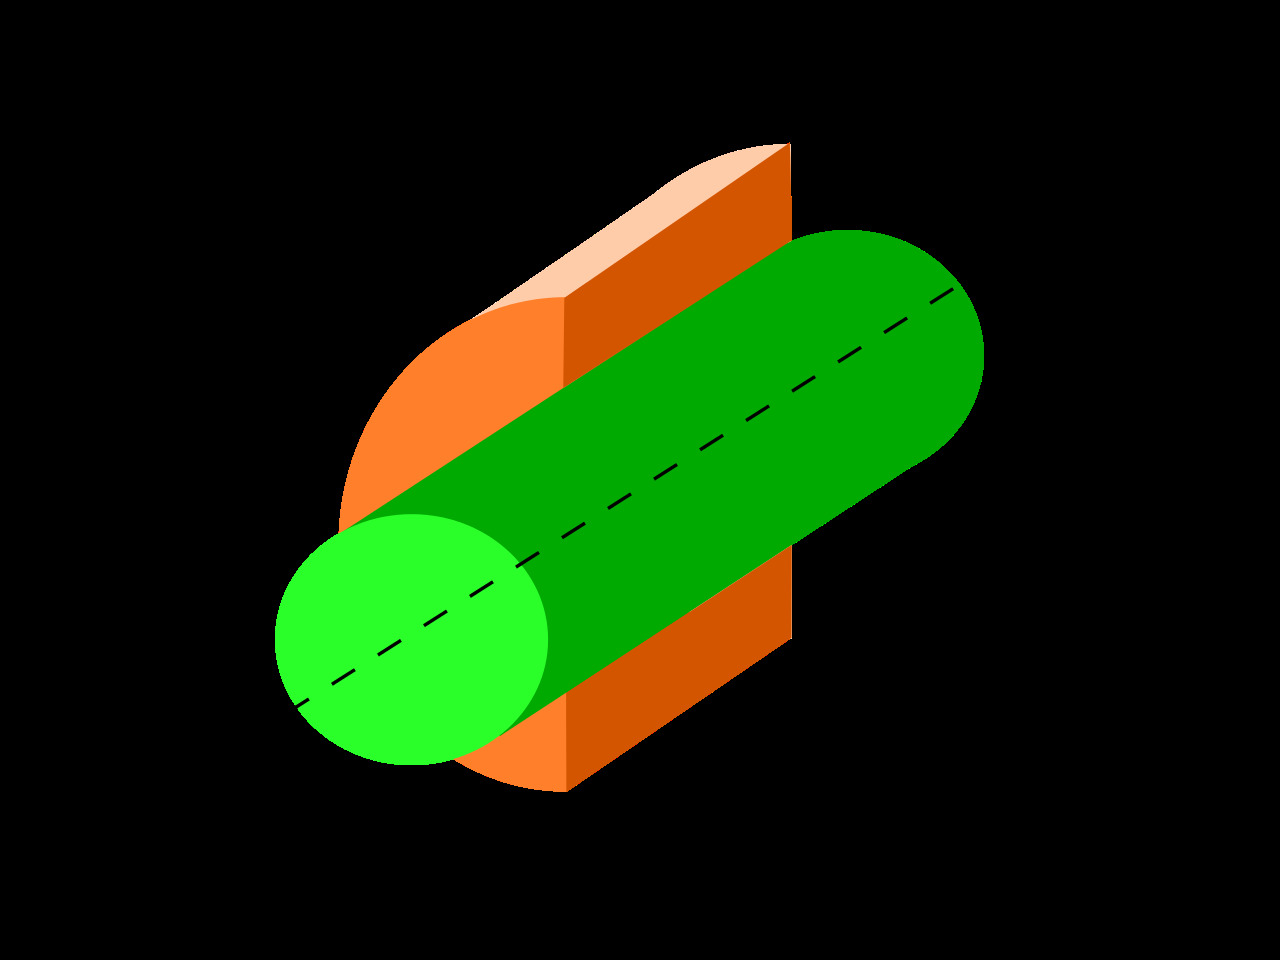
\includegraphics[width=\textwidth]{figures/revolute.jpg}
			\end{figure}
		\end{column}
		\begin{column}{.5\textwidth}
			\begin{figure}
				\centering
				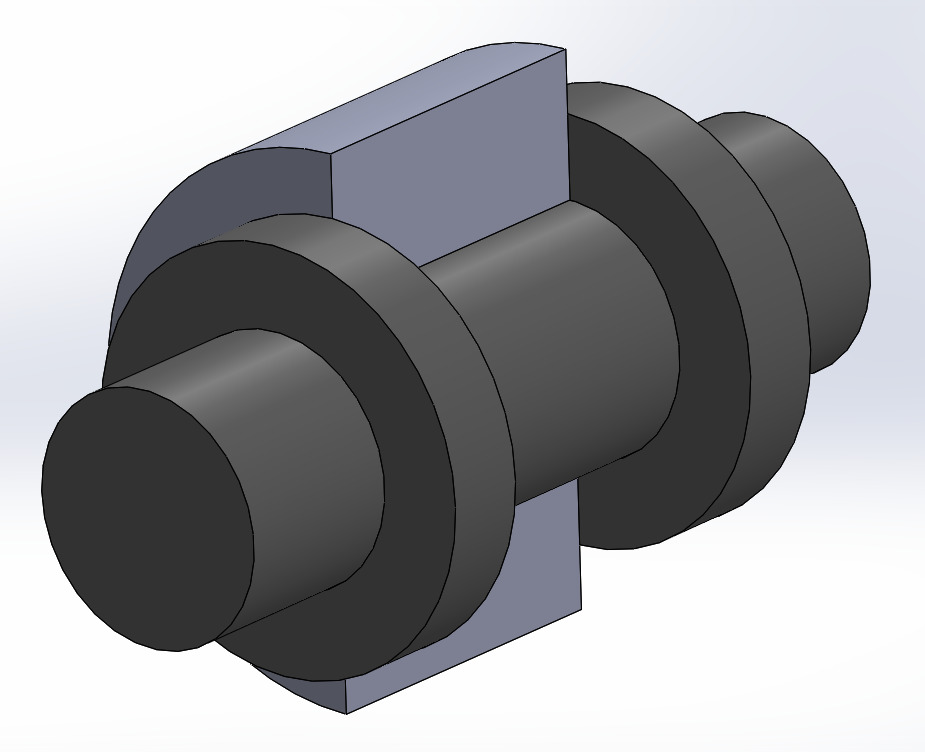
\includegraphics[width=\textwidth]{figures/revolute_cutaway.jpg}
			\end{figure}
		\end{column}
	\end{columns}
	%
	 \footnotesize{\textcolor{red}{Revolute} or \textcolor{red}{Hinge} or \textcolor{red}{Turning} or simply \textcolor{red}{$R$-pairs} with and without shoulder cutaway geometries. Credit: Wikimedia commons.}
\end{frame}


\begin{frame}
	\frametitle{Helical- \& U-Joints}
	%
	\begin{columns}[t]		
		\begin{column}{.5\textwidth}
			\begin{figure}
				\centering
				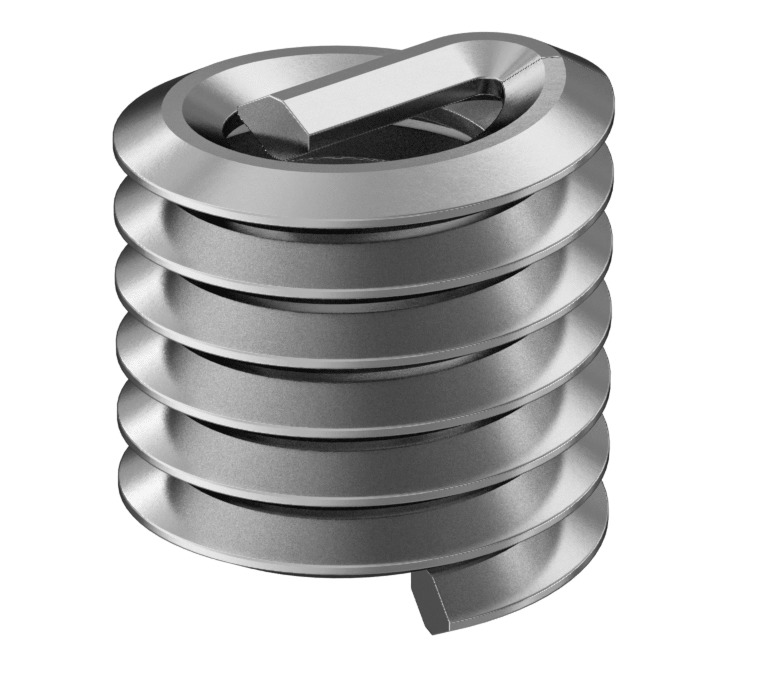
\includegraphics[width=\textwidth]{figures/helical.jpg}
			\end{figure}
			\centering Helical Joint
		\end{column}	
		\begin{column}{.5\textwidth}
			\begin{figure}
			\centering
			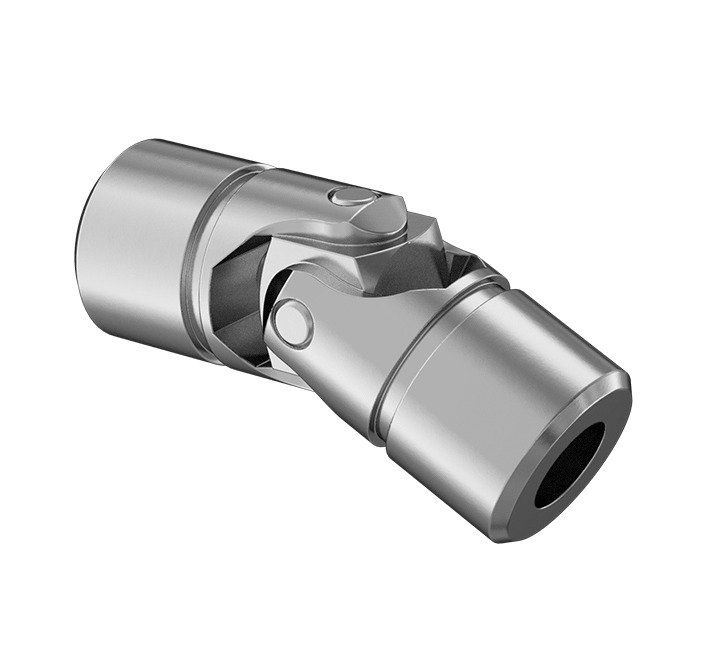
\includegraphics[width=\textwidth]{figures/ujoint.jpg}
			\end{figure}
			\centering Universal Joint
		\end{column}
	\end{columns}
	%
	\footnotesize{\copyright McMaster Carr, May 2022.}
\end{frame}


%\note{Introduce the concept of lower and higher pairs. Then explain a linkage.}



\begin{frame}
	\frametitle{Common Lower Kinematic Pairs}
	%
	\begin{figure}[t]
		\centering
		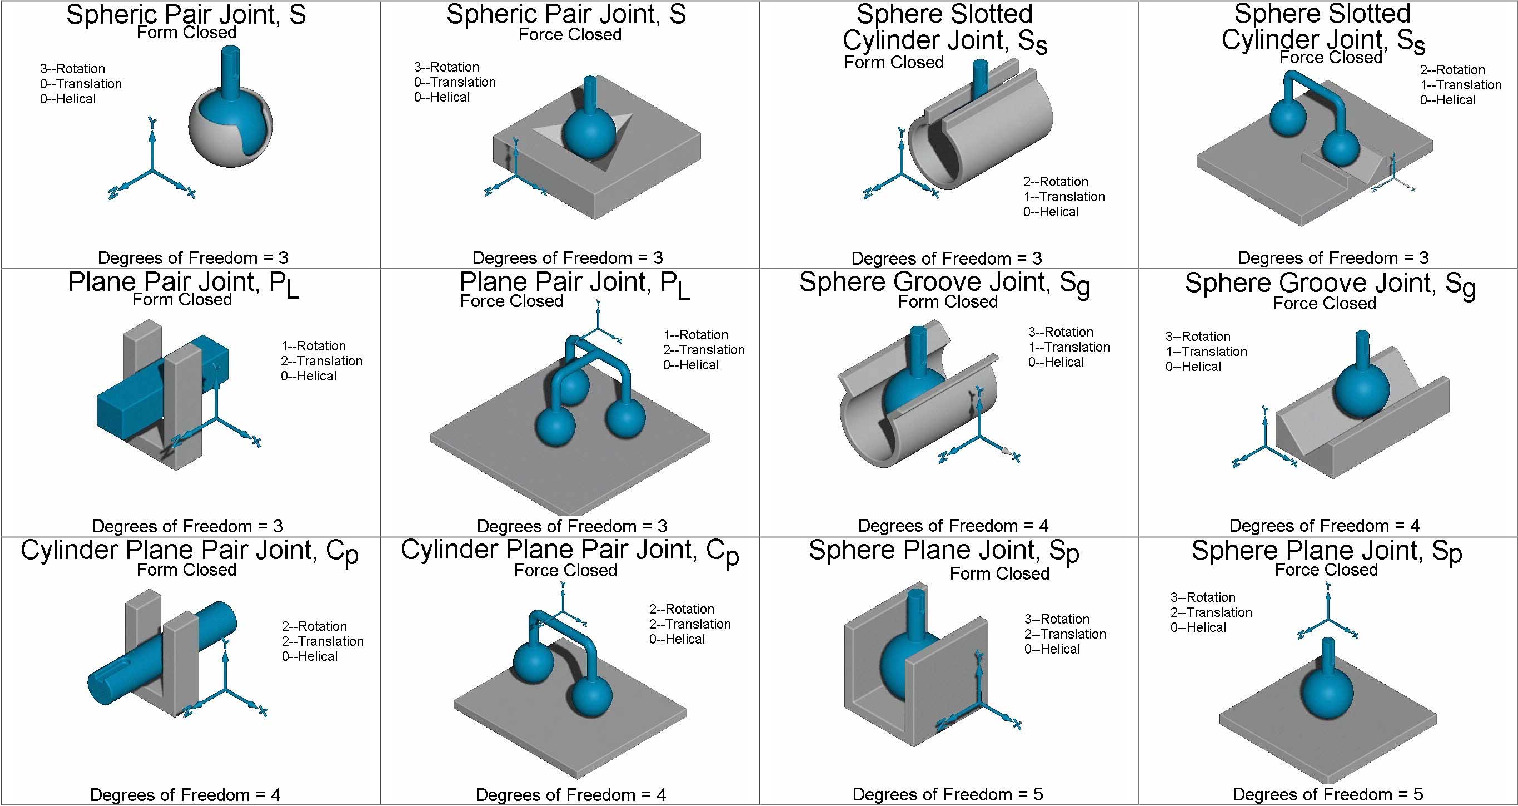
\includegraphics[width=\columnwidth]{figures/pairs2.jpg}
		Credit: \href{https://www.semanticscholar.org/paper/Development-of-Solid-Models-and-Multimedia-of-Pairs-Wharton-Singh/7ba9c2f3cfed5a493bb5828976689764d024b087}{\textcolor{blue}{Wharton and Singh,  2001}}.
	\end{figure}
\end{frame}


\begin{frame}
	\frametitle{Common Lower Kinematic Pairs}
	%
	\begin{figure}[t]
		\centering
		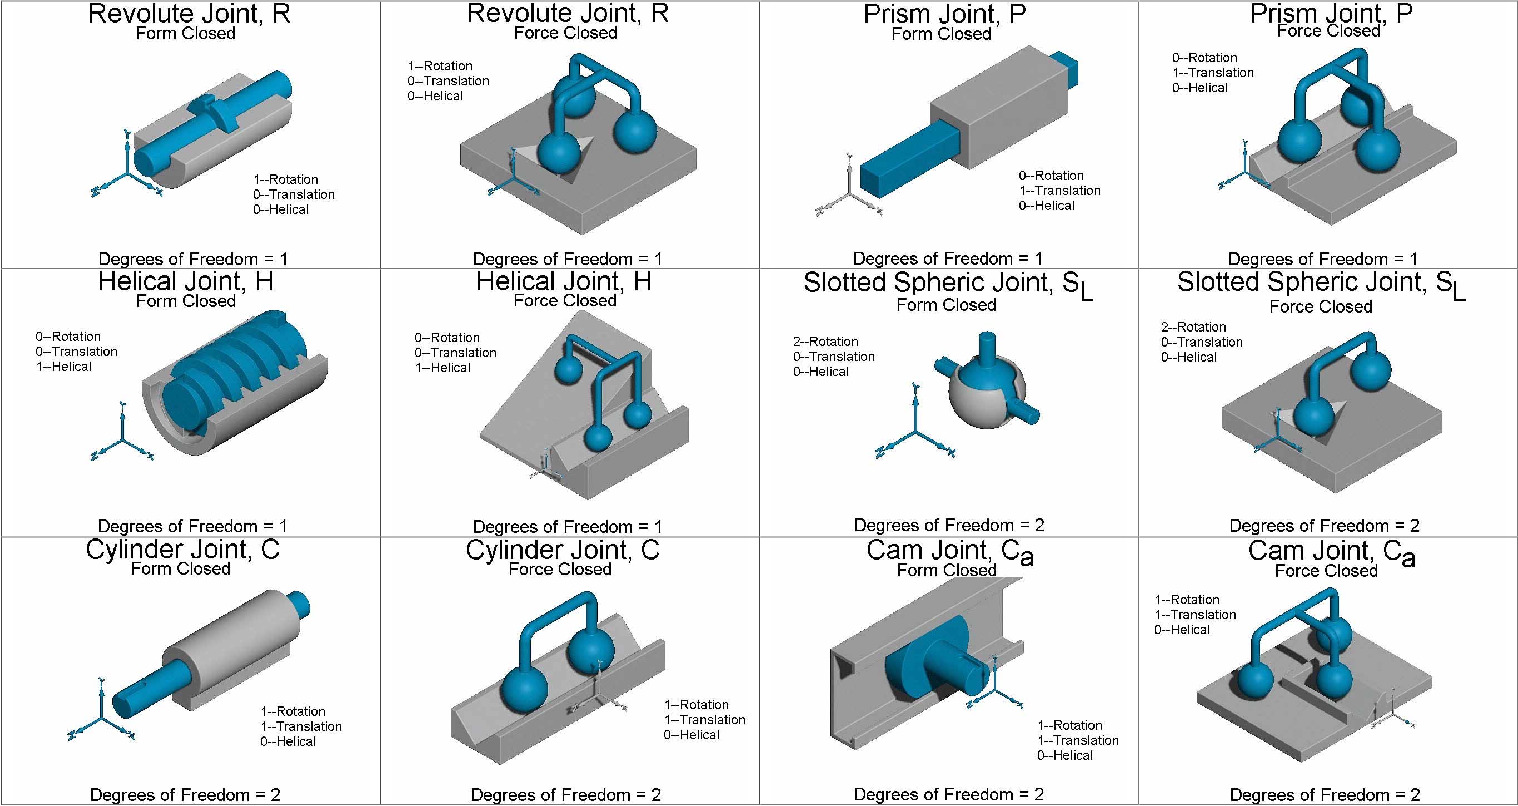
\includegraphics[width=\columnwidth]{figures/pairs.jpg}
		Credit: \href{https://www.semanticscholar.org/paper/Development-of-Solid-Models-and-Multimedia-of-Pairs-Wharton-Singh/7ba9c2f3cfed5a493bb5828976689764d024b087}{\textcolor{blue}{Wharton and Singh,  2001}}.
	\end{figure}
\end{frame}
	
	
\begin{frame}
	\frametitle{Kinematic Geometry of Common Actuations}
	\begin{block}{In-series vs. Parallel-actuated lower pairs}
		\begin{columns}[t]
			\begin{column}{10cm}
				\centering
				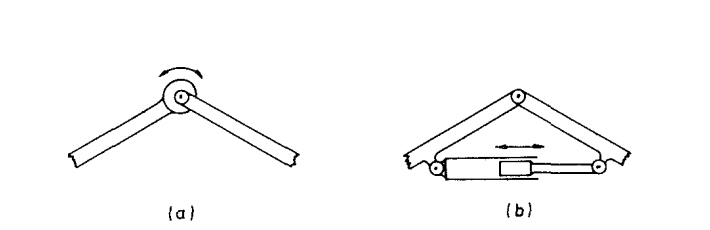
\includegraphics[width=\textwidth]{../Notes/figures/arms_hunt.png}
			\end{column}
		\end{columns}
		\footnotesize{(a): In-series-actuated kinematic pair with a rotary joint that is actuated ``about" the hinge. (b): Prismatic joint actuated ``across" a hinge. Reprinted from Hunt, Kenneth. Structural Kinematics of In-Parallel-Actuated Robot Arms. Transactions of ASME. 1983. }
	\end{block}
\end{frame}
		
\begin{frame}
	\frametitle{Kinematic Chains}
	%	
	\begin{block}{Kinematic Chains (Reuleaux, 1975)}
			We can explain the structural similarity of many mechanisms by parts of \textcolor{red}{kinematic chains} connected by pairs.
	\end{block}
	\begin{block}{Kinematic chains}
		\textcolor{blue}{Kinematic chains} are essentially the basic building structure of \textcolor{red}{mechanisms} $\ldots$ \textcolor{red}{and robots!} 
	\end{block}
\end{frame}
	
%\begin{frame}
%		\frametitle{Kinematic Chains}
%		%\begin{block}{.5\textwidth}
%		\begin{columns}[t]
%			\begin{column}{5cm}
%					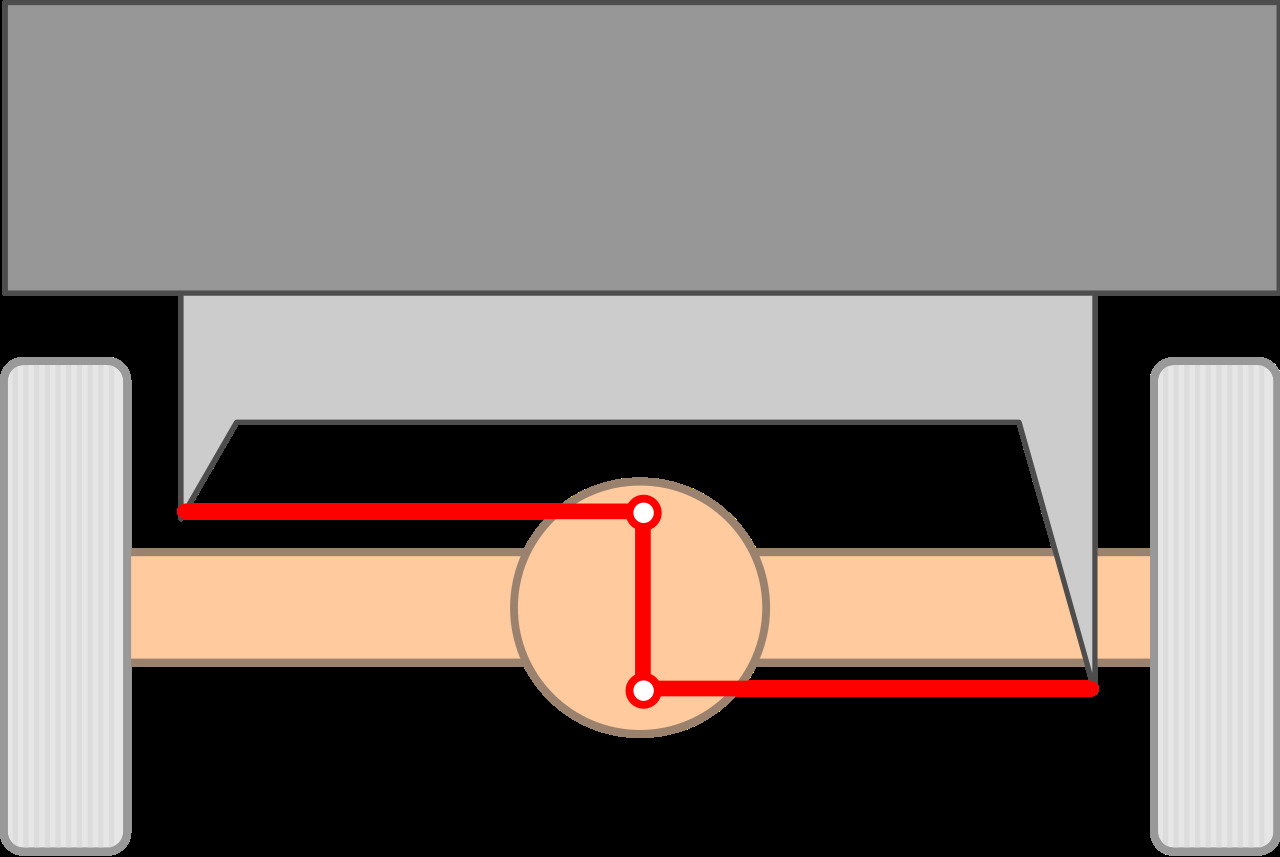
\includegraphics[width=1.5\textwidth, height=1.5\textwidth]{figures/WattsLinkage.jpg} 
%					\footnotesize{The Watt's Linkage Vehicle Suspension.} 
%		\end{column}
%			%	
%		\begin{column}{5cm}
%			\begin{minipage}[b]{.5\textwidth}
%				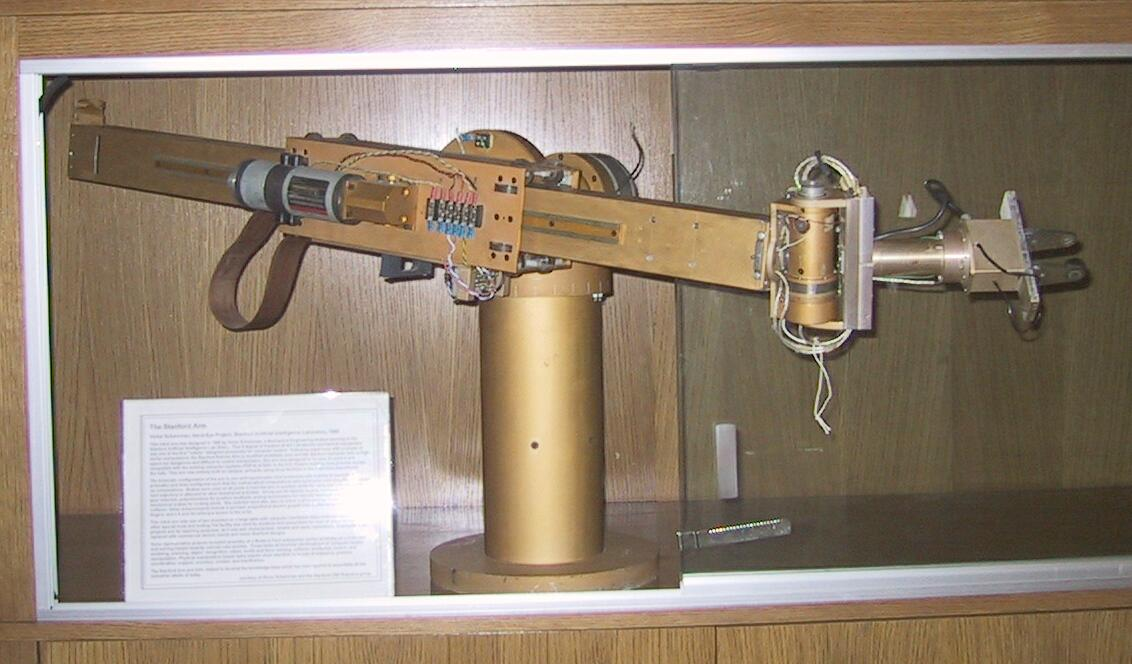
\includegraphics[width=1.5\textwidth, height=1.5\textwidth]{../Notes/figures/StanfordArm.jpg}  \\
%				\footnotesize The Stanford Arm (Infolab 1969). %Six degrees of freedom open kinematic chain.
%			\end{minipage}
%		\end{column}
%	\end{columns}
%%\end{block}
%\end{frame}

\subsection{Serial Chains}
	\begin{frame}
		\frametitle{Open Kinematic Chains}
		%	
		\begin{block}{Chains}
			Open kinematic chains are based off the anthropomorphic construction of the human hand with cantilevered beam structures.
		\end{block}
		\begin{block}{Chain Mechanisms and Error Amplification}
			Amplifies errors from waist (or base frame) all the way to the tool frame. Control difficult. 
		\end{block}
		%
		\begin{block}{Control}
			Feedforward control: High power and precision hydraulic actuators for servo motors. \\
			Sensory feedback control: Force sensing (Ernst, 1962). 
		\end{block}
	\end{frame}
	
	
	\note{The PUMA arm is the world's first serial kinematic chain. Developer: Victor Scheinman, Stanford student in the `50's. Made several iterations. Patent Rights: Joe Engelberger, (Danbury Unimation, 1961). Joe -- father of robotics -- created world's first robotics company in '61.}
	\begin{frame}
		\frametitle{Open Kinematic Lower Pairs}
		\begin{definition}[Ken Salisbury Jr., 1982]
			``\footnotesize \textit{[Robots are] our fascination with constructing mechanical analogues of ourselves... [this fascination] has led us to place all sorts of hopes and expectations in robot capabilities}."
		\end{definition}
		\begin{columns}[t]
			\begin{column}{5cm}
				\begin{minipage}[b]{.5\textwidth}
					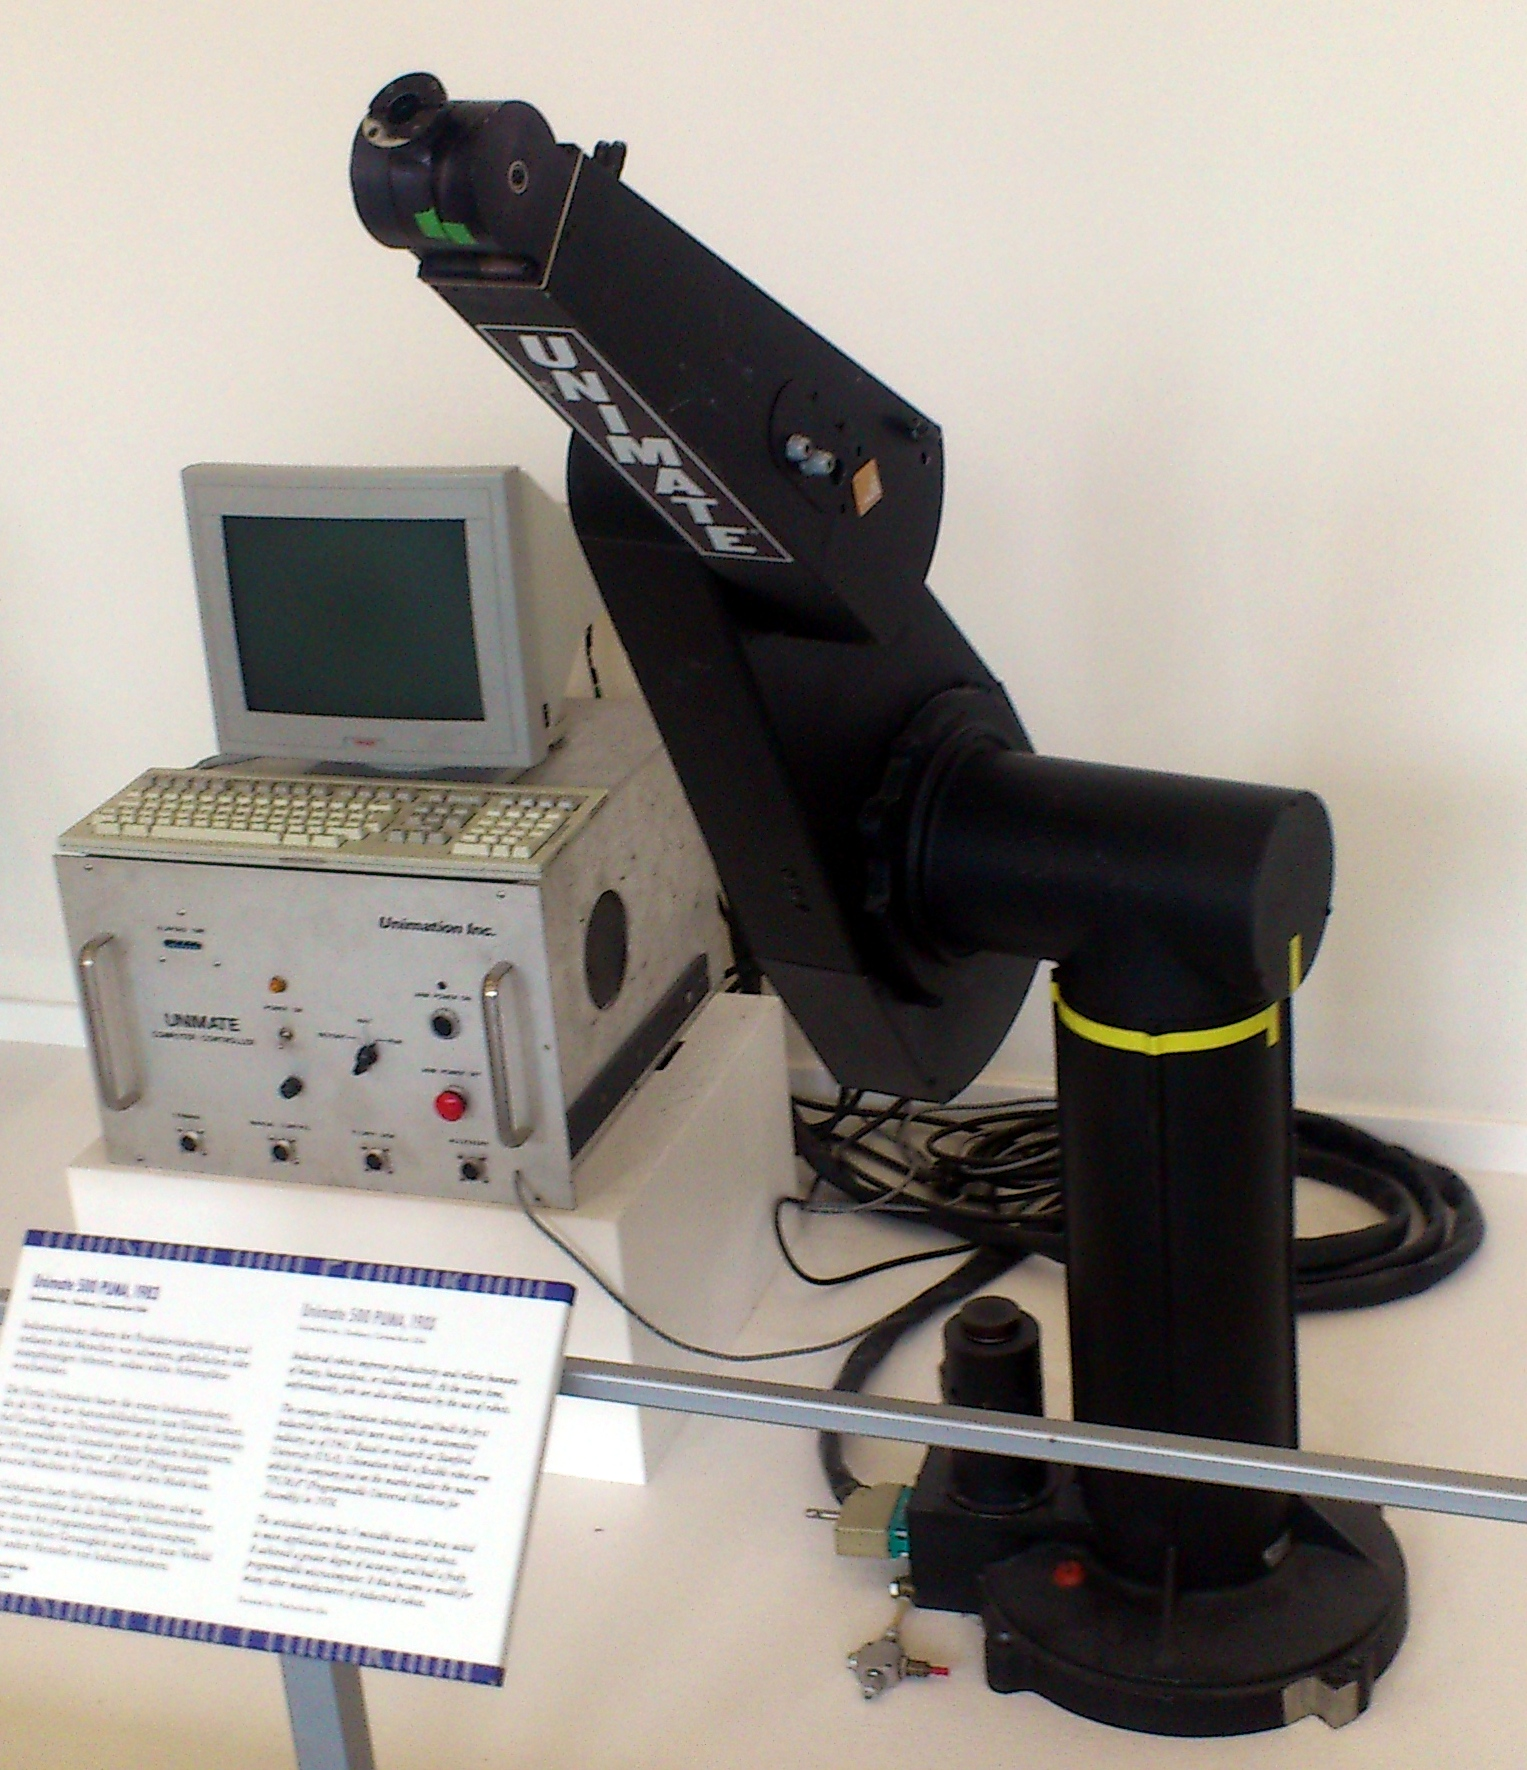
\includegraphics[width=1.5\textwidth, height=1.5\textwidth]{../Notes/figures/PUMA.jpg} \\
					\footnotesize{The PUMA Robot (1956).} %Programmable Universal Manipulation Arm.}
			\end{minipage}
			%
		\end{column}	
		\begin{column}{5cm}
			\begin{minipage}[b]{.5\textwidth}
				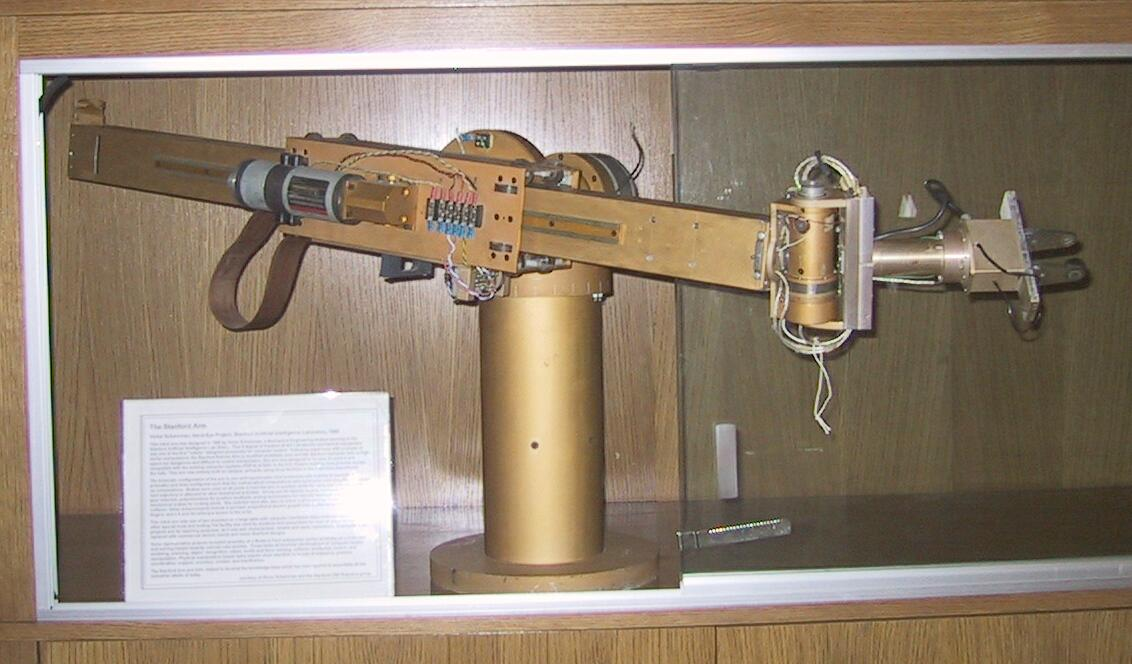
\includegraphics[width=1.5\textwidth, height=1.5\textwidth]{../Notes/figures/StanfordArm.jpg}  \\
				\footnotesize The Stanford Arm (Infolab 1969). %Six degrees of freedom open kinematic chain.
			\end{minipage}
		\end{column}
	\end{columns}
\end{frame}


\begin{frame}
\frametitle{Open Kinematic Chains}
%
\begin{tcolorbox}[coltitle=blue!80!yellow,colframe=brown!80]
	Open kinematic chains provide unstructured environmental interaction.
\end{tcolorbox}
\begin{tcolorbox}[coltitle=blue!80!yellow,colframe=gray!100]
	Project MAC, MIT.
\end{tcolorbox}
\begin{tcolorbox}[coltitle=blue!80!yellow,colframe=black!80]
	Tomovic and Boni's pressure sensed grasp.
\end{tcolorbox}
\begin{tcolorbox}[coltitle=blue!80!yellow,colframe=pink!100]
	Binary robot vision system (McCarthy et al, 1963).
\end{tcolorbox}
\end{frame}

\begin{frame}
\frametitle{Open Kinematic Chains}
%
\begin{tcolorbox}[coltitle=cyan!80,colframe=green!100]
	Stanford Manipulator.
\end{tcolorbox}
\begin{tcolorbox}[coltitle=blue!80!yellow,colframe=blue!100]
	Boston arm.
\end{tcolorbox}
\begin{tcolorbox}[coltitle=blue!80!yellow,colframe=red!100]
	The AMF (American Machines and Foundry) arm.
\end{tcolorbox}
\begin{tcolorbox}[coltitle=blue!80!yellow,colframe=yellow!100]
	General electric's walking robot (1969).
\end{tcolorbox}
\end{frame}


\begin{frame}
\frametitle{Long Walk Towards Direct Drive Robot Arms}

\begin{tcolorbox}[coltitle=magenta!80!green,colframe=yellow!80!green]
	The 50's, 60's nd 70's witnessed use of hydraulics  for (feedforward) position control.
\end{tcolorbox}

\begin{tcolorbox}[coltitle=magenta!80!green,colframe=blue!80!green] 
	For feedback control, force sensors and pressure sensors were used in closed-loop scenarios.
\end{tcolorbox}

\begin{tcolorbox}[coltitle=magenta!80!green,colframe=red!80!green] 
	Electrical actuation meant that robots had to be operated at high speeds. Needs for gear reduction for safe operations at low speeds. 
\end{tcolorbox}

\begin{tcolorbox}[coltitle=magenta!80!green,colframe=brown!80!green]
	With gear reduction came backlash, friction, and associated expenses.
\end{tcolorbox}
\end{frame}


\note{CMU DD I/II Arms: Workspace is donut shaped. OD:  90cm; ID: 21.7cm; $1.8m^2$ workspace area. Built by Harry Asada. Structural design similar to aircraft gimbal arm; Uses Samarium Cobalt rare earth magnet brushless DC motors on first 3 joints, and AlNiCo magnets on tip joints. No belts, transmissions making for faster transmitting of motions, less friction, low energy, low compliance. Each joint has complex AL housing which enables: (i) Control of geometrical relationships of bearing assembly; (ii) Control of servo components to bearing assembly; (iii) Controls of rotational axes to consecutive joints.}


\begin{frame}
\frametitle{Direct Drive Robot Mechanism: CMU DD I Arm}
\begin{tcolorbox}[coltitle=blue!80!yellow,colframe=brown!80!green]
	Along came Harry Asada.
\end{tcolorbox}
\begin{columns}[t]	
	%
	\begin{column}{.45\columnwidth}
		\begin{minipage}[b]{\textwidth}
			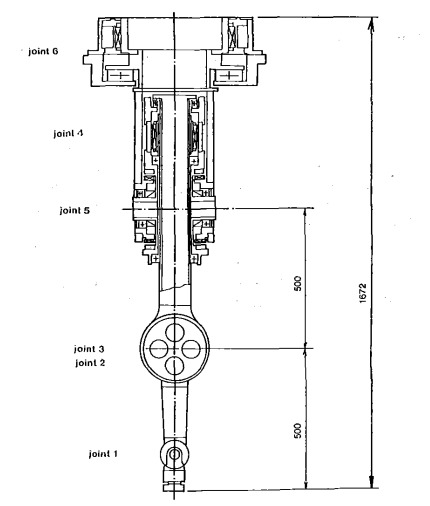
\includegraphics[width=1.2\textwidth, height=1.2\textwidth]{figures/cmu_arm.jpg} \\
			\footnotesize{Arm Schematics Transmission} %Programmable Universal Manipulation Arm.}
	\end{minipage}
	%
\end{column}
%
\begin{column}{.45\columnwidth}
	\begin{minipage}[b]{\textwidth}
		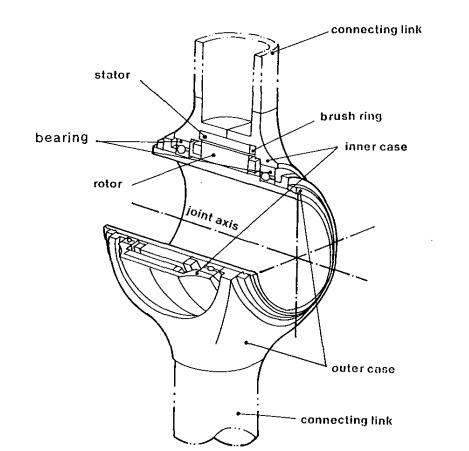
\includegraphics[width=1.2\textwidth, height=1.2\textwidth]{figures/dd_joints.jpg} \\
		\footnotesize{Joint schematic} %Programmable Universal Manipulation Arm.}
\end{minipage}
%
\end{column}
\end{columns}
\end{frame}

\begin{frame}
\frametitle{Direct Drive Robot Mechanism: CMU DD I Arm}
\begin{columns}[t]					%
%
\begin{column}{.45\columnwidth}
\begin{minipage}[b]{\textwidth}
	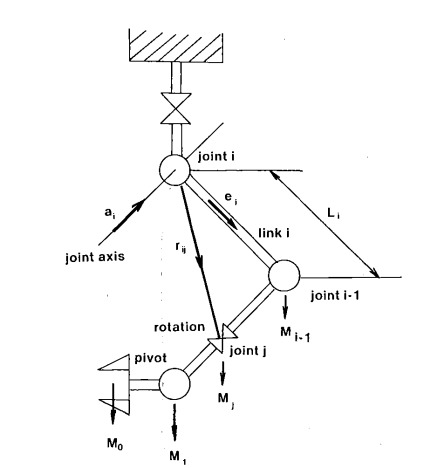
\includegraphics[width=1.1\textwidth, height=1.5\textwidth]{figures/dd_kinematics.jpg} \\
	\footnotesize{Kinematic model} %Programmable Universal Manipulation Arm.}
\end{minipage}
%
\end{column}
\begin{column}{.45\columnwidth}
\begin{minipage}[b]{\textwidth}
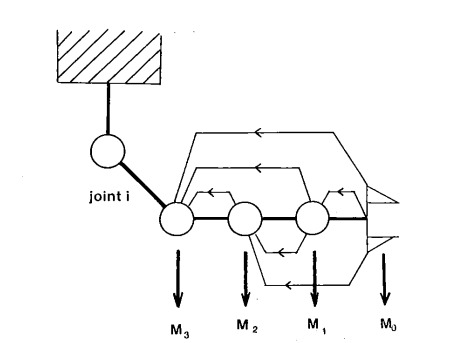
\includegraphics[width=1.2\textwidth, height=1.5\textwidth]{figures/dd_load_joints.jpg} \\
\footnotesize{Errors Transmission} %Programmable Universal Manipulation Arm.}
\end{minipage}
\end{column}
\end{columns}\end{frame}


\note{First direct-drive robot without a gearbox. Selective compliance in X-Y directions given its articulated jointed arms. One-freedom motion along $Z$ direction given its constrained arm New generations such as Cobra i600/i800 include power amplifiers, system and servo controls etc embedded in the robot's base. Kuka Scara arm: Lightweight, fast, powerful, low maintenance, energy consumption, investment costs etc.}
\begin{frame}
\frametitle{SCARA Robot Mechanisms}
\begin{columns}[t]	
\begin{column}{5cm}
\begin{minipage}[b]{.5\textwidth}
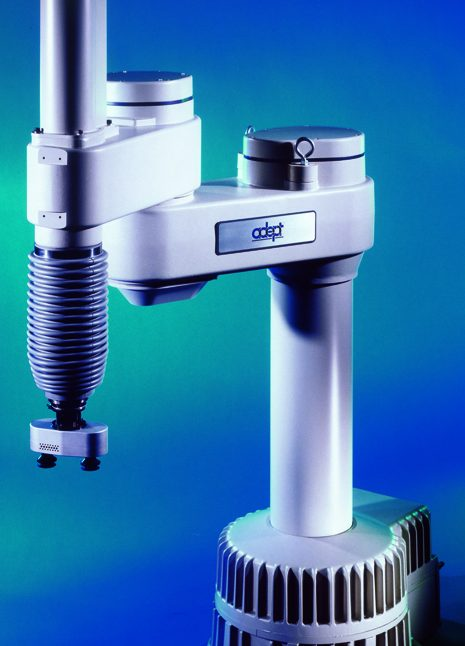
\includegraphics[width=1.5\textwidth, height=1.5\textwidth]{figures/adeptone.jpg}  \\
\footnotesize The Adept One SCARA robot (Debuted 1984). 
\end{minipage}
\end{column}
%
\begin{column}{5cm}
\begin{minipage}[b]{.5\textwidth}
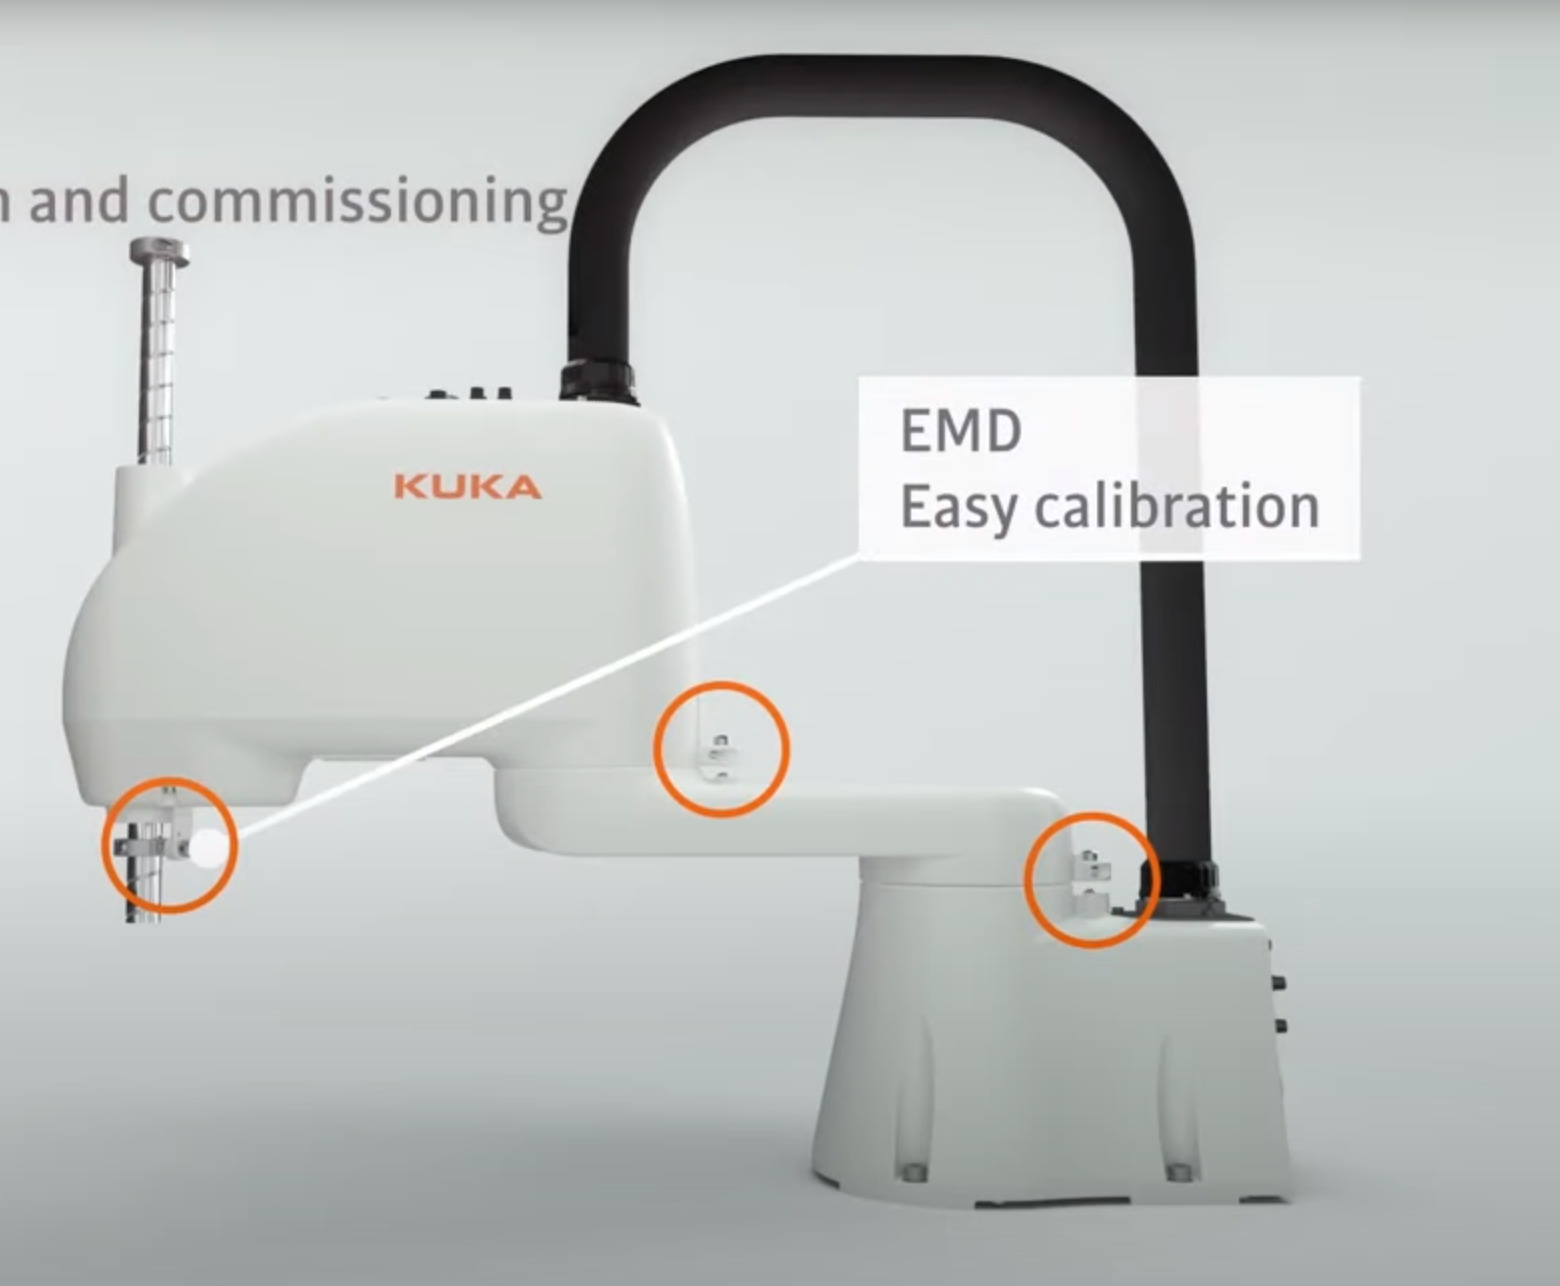
\includegraphics[width=1.5\textwidth, height=1.5\textwidth]{figures/Scara.jpg} \\
\footnotesize{Kuka's SCARA arm, 2022. \copyright Kuka Robotics} %Programmable Universal Manipulation Arm.}
\end{minipage}
%
\end{column}
\end{columns}
\end{frame}


\begin{frame}
	\begin{block}{The St{\"a}ubli anthropomorphic arm.}
		\begin{columns}[t]
			\begin{column}{10cm}
				\centering
				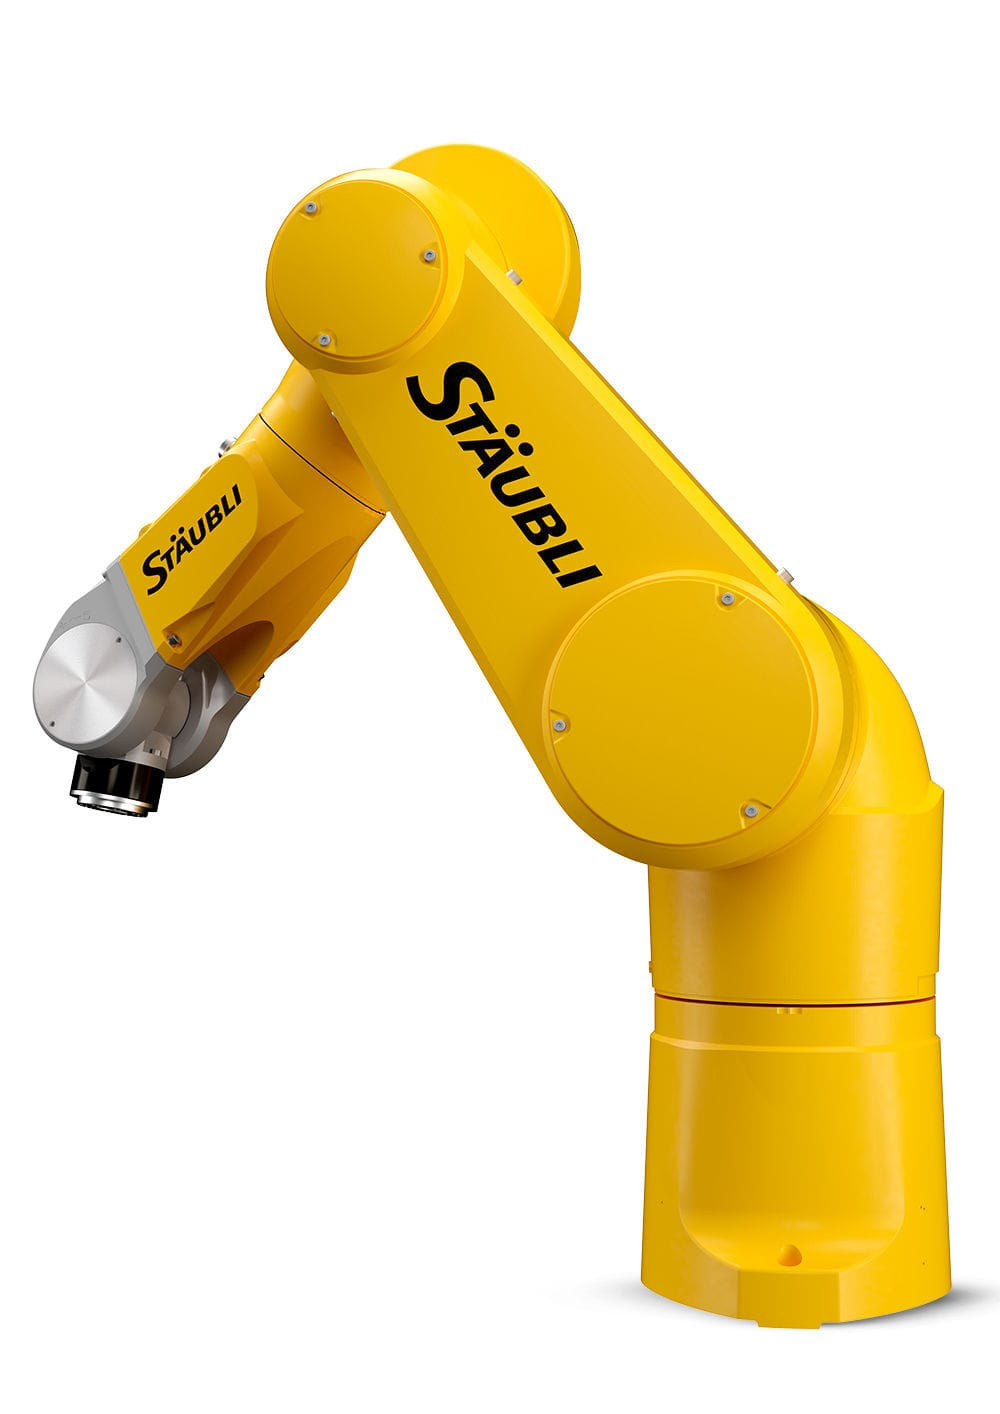
\includegraphics[scale=.1, width=.5\textwidth, rotate=0]{../Notes/figures/Staubli.jpg}
			\end{column}
		\end{columns}
		\footnotesize{The Staubli 6-DOF Arm is an example of a Spherical Manipulator. Reprinted from DirectIndustry's Webpage.}
	\end{block}
\end{frame}

\begin{frame}
\frametitle{Serial mechanisms research in the 80's}
%
\tcbset{coltitle=cyan!80,colframe=gray!80!green,title=Mechanisms in the 80's,
enlarge left by=-5mm,enlarge right by=0mm,width=\linewidth+5mm}
\begin{tcolorbox}[toggle enlargement=none]
With the 80's came the arrival of PCs. Lots of research went into computational algorithms for the kinematics and kinetics of (mostly) anthropomorphic robot arms.
\end{tcolorbox}
\begin{tcolorbox}[coltitle=magenta!70,colframe=blue!80!red,title=Active control schemes,toggle enlargement=forced]
Efficient recursive Lagrangian and computational methods for the gravitational and Coriolis forces in Newton-Euler equations.
\end{tcolorbox}
\end{frame}

\begin{frame}
	\frametitle{Serial mechanisms research in the 80's}
	%
	\tcbset{coltitle=cyan!80,colframe=gray!80!green,title=Mechanisms in the 80's,
		enlarge left by=-5mm,enlarge right by=0mm,width=\linewidth+5mm}
	\begin{tcolorbox}[coltitle=pink!70,colframe=gray!80!red,title=Feedback Linearization,toggle enlargement=evenpage]
		Dynamics feedback linearization for precise bounds on manipulator performance.
	\end{tcolorbox}
	
	\begin{tcolorbox}[title=Automatix,toggle enlargement=none]
		Reconfigurable robots for various assembly ops.
	\end{tcolorbox}
\end{frame}

\begin{frame}
\frametitle{Serial mechanisms research in the 90's}
%
\tcbset{coltitle=pink!80,colframe=gray!80,title=Robotworld,
enlarge left by=-5mm,enlarge right by=0mm,width=\linewidth+5mm}
\begin{columns}[b]
\begin{column}{.48\columnwidth}			
\begin{tcolorbox}[colframe=blue!80!green, coltitle=white!80,toggle enlargement=none]
First industrial-scale re-configurable robot and with machine vision components. RAIL scripting OS originally based on Motorola 68000, later on replaced by Apple Macintosh II. 
\end{tcolorbox}
\end{column}
\begin{column}{.52\columnwidth}
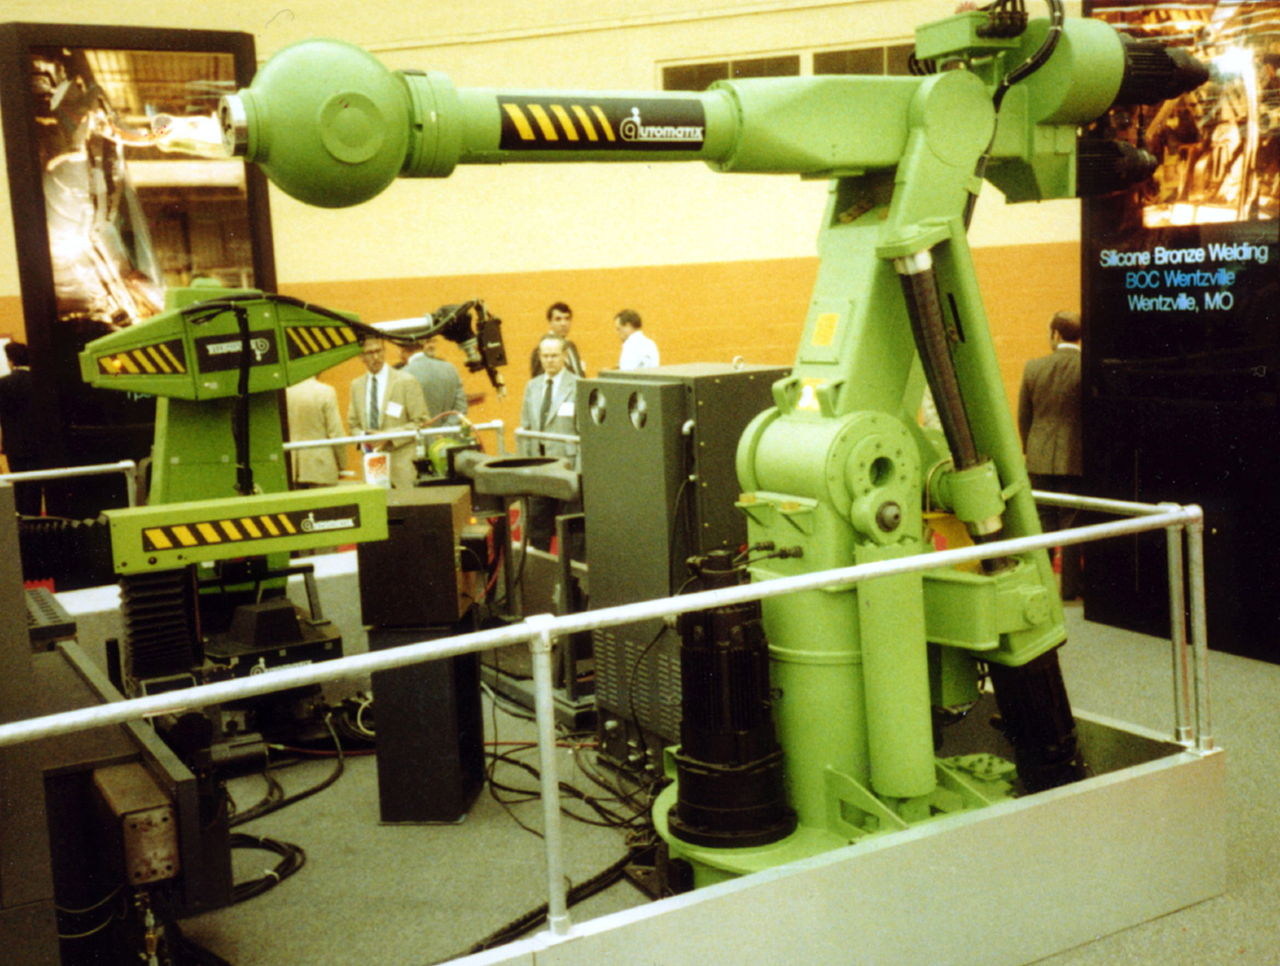
\includegraphics[width=\textwidth]{figures/Automatix.jpg}
\copyright Wikipedia
\end{column}
\end{columns}
\end{frame}

\subsection{Hyperredundant and Parallel robots}
	\begin{frame}
		\frametitle{Hyper-redundant Continuum Robots}
		\begin{columns}[b]
			\begin{column}{.33\columnwidth}			
				\begin{tcolorbox}[colframe=blue!80!green, coltitle=white!80,toggle enlargement=none]
					\centering 
					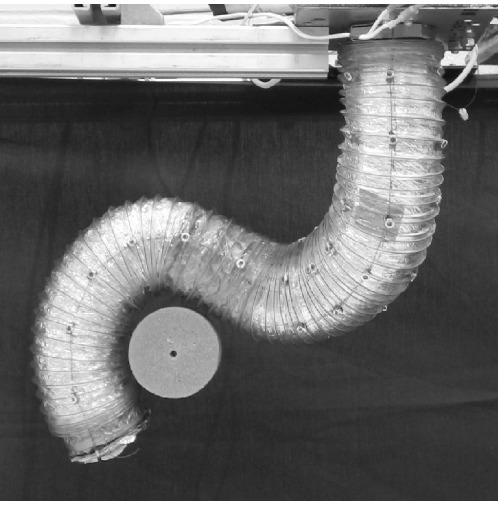
\includegraphics[width=\textwidth, height=1.1\textwidth]{figures/multisec_continuum.jpg}
				\end{tcolorbox}
			\end{column}	
		\begin{column}{.33\columnwidth}			
			\begin{tcolorbox}[colframe=blue!80!green, coltitle=white!80,toggle enlargement=none]
			\centering 
			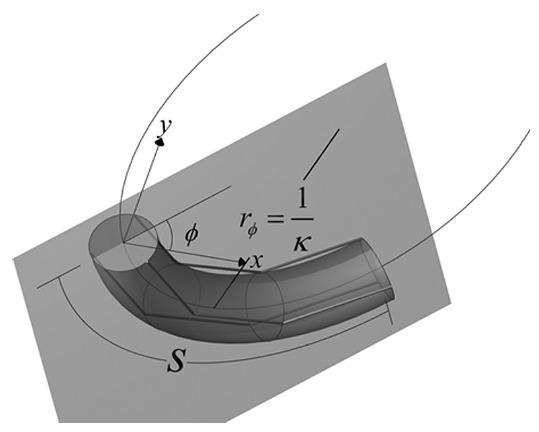
\includegraphics[width=\textwidth, height=1.1\textwidth]{figures/multi_sec_manip.jpg}
			\end{tcolorbox}
		\end{column}	
		\begin{column}{.33\columnwidth}			
			\begin{tcolorbox}[colframe=blue!80!green, coltitle=white!80,toggle enlargement=none]
			\centering 
			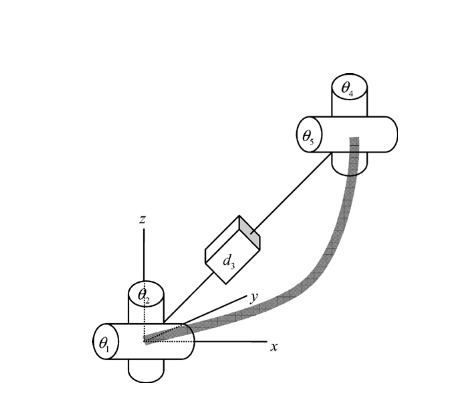
\includegraphics[width=\textwidth, height=1.1\textwidth]{figures/multi_sec_scheme.jpg}
			\end{tcolorbox}
		\end{column}	
		\end{columns}
		\centering \footnotesize{The elephant trunk continuum robot. Jones \& Walker, T-RO 2006. Inspiration: Muscular hydrostats in nature.}
	\end{frame}

\begin{frame}
	\frametitle{Hyper-redundant Kinematic Chains}
	\begin{columns}[b]
		\begin{column}{.98\columnwidth}			
			\begin{tcolorbox}[colframe=blue!80!green, coltitle=white!80,toggle enlargement=none]
				\centering 
				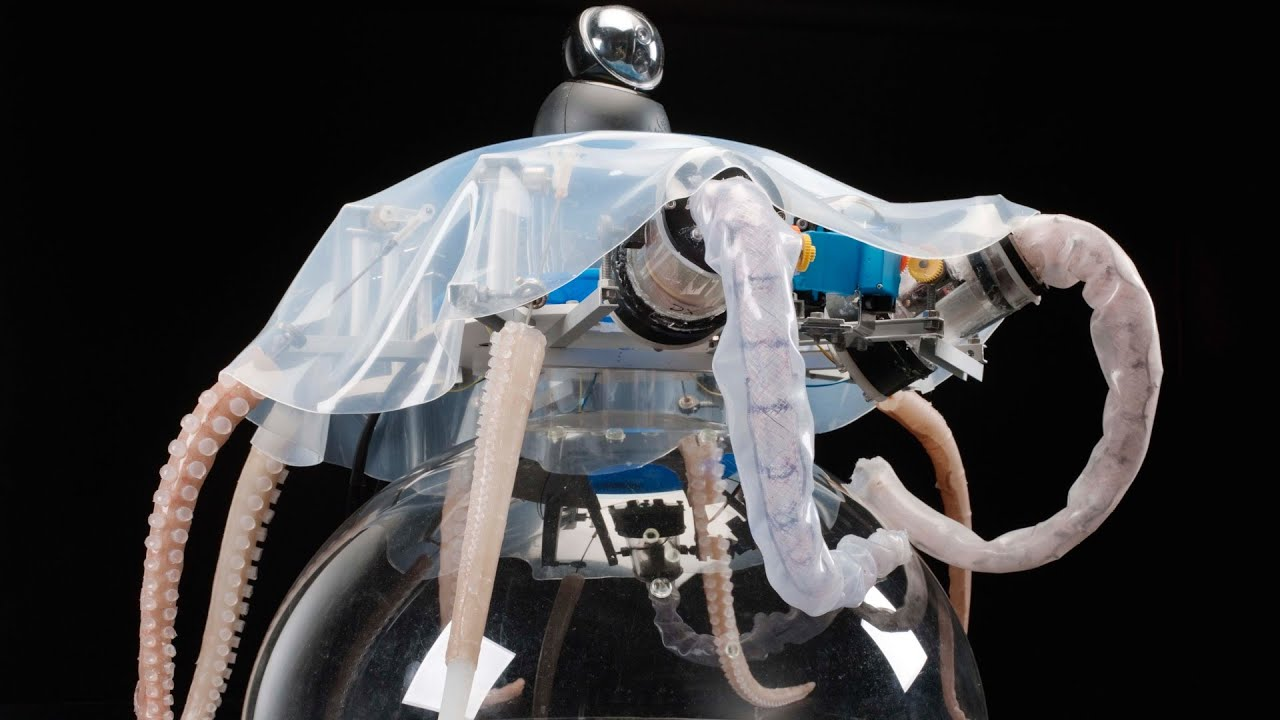
\includegraphics[width=\textwidth]{../Notes/figures/octopus.jpg}
			\end{tcolorbox}
		\end{column}	
	\end{columns}
	 \centering \footnotesize{An octopus-inspired soft robot. \copyright Cecilia Laschi.}
\end{frame}
	
	
	\begin{frame}
		\frametitle{Parallel Robots}
		%
		\tcbset{coltitle=light-blue!100,colframe=cyan!50,title=Robotworld,
			enlarge left by=-5mm,enlarge right by=0mm,width=\linewidth+5mm}
		\begin{tcolorbox}[title=Mehlet 2015,toggle enlargement=none]
			A \textcolor{blue}{parallel robot} is made up of an end-effector with $n$ degrees of freedom, and of a fixed base, linked together by at least two independent kinematic chains. Actuation takes place through n simple actuators.
		\end{tcolorbox}	
	\end{frame}
	
	\begin{frame}
		\frametitle{Parallel mechanisms: Stewart-Gough Platforms}
		\footnotesize{Principles of a moving platform to test tyre wear and tear (Gough, 1947). Prototype, 1955.}
		\newline
		\begin{columns}[b]
			\begin{column}{.48\columnwidth}			
				\begin{tcolorbox}[colframe=blue!80!green, coltitle=white!80,toggle enlargement=none]
					\centering 
					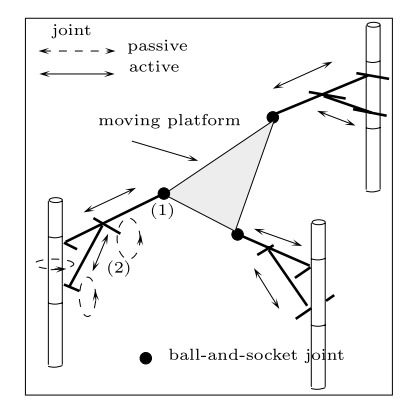
\includegraphics[width=\textwidth]{figures/Stewart.jpg}
				\end{tcolorbox}
			\end{column}
			\begin{column}{.48\columnwidth}			
				\begin{tcolorbox}[colframe=blue!80!green, 	coltitle=white!80,toggle enlargement=none]
				\centering 
				\includegraphics[width=.8\textwidth]{../../../Papers/PhDThesis/figures/GoughPlatform.jpg}
				\end{tcolorbox}
			\end{column}	
		\end{columns}
		\centering \footnotesize{\textit{Left}: Stewart's 1965 mechanism. \textit{Right:} The original 1954 octahedral hexapod proposed by  Gough. Courtesy: Parallemic.org.}
	\end{frame}

\begin{frame}
	\frametitle{Truss Robots}
	\begin{columns}[b]
		\begin{column}{.7\columnwidth}			
			\begin{tcolorbox}[colframe=blue!80!green, coltitle=white!80,toggle enlargement=none]
				\centering 
				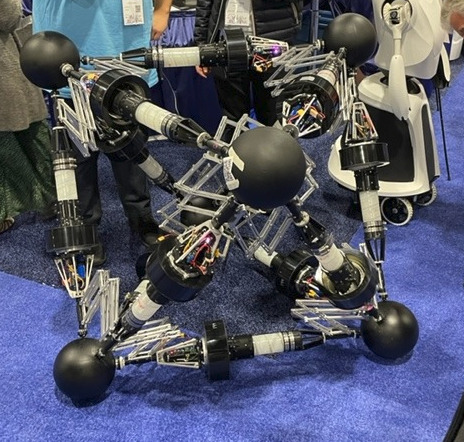
\includegraphics[width=.8\textwidth]{figures/truss.jpg}
			\end{tcolorbox}
		\end{column}	
	\end{columns}
	\centering \footnotesize{A multi-DOF Truss Robot. Courtesy of Penngineering (ICRA 2022, Philadelphia, PA).}
\end{frame}		
		
\begin{frame}
	\frametitle{Closed kinematic chains}
	\footnotesize{Connection degree $\ge 3$.}
	\newline
		\begin{columns}[b]
			\begin{column}{.74\columnwidth}			
				\begin{tcolorbox}[colframe=blue!80!green, coltitle=white!80,toggle enlargement=none]
					\centering 
					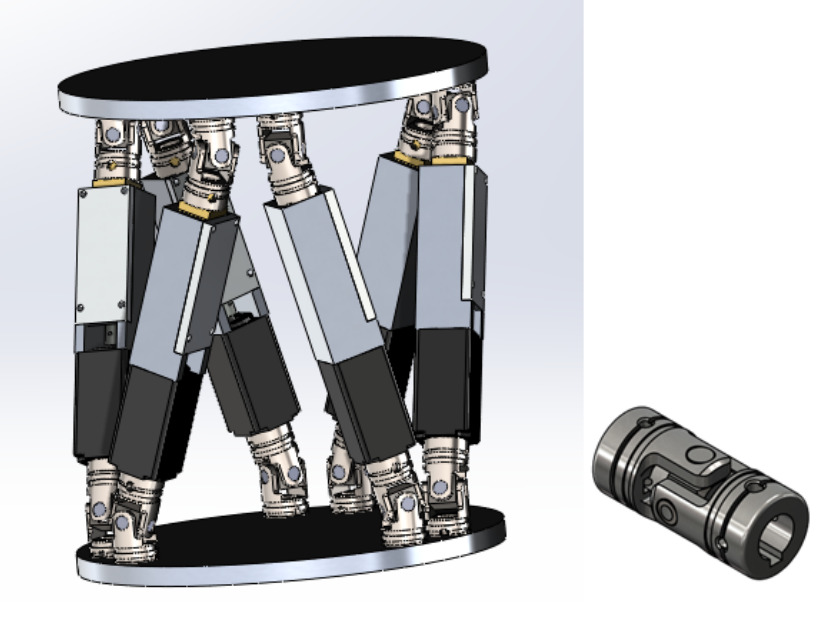
\includegraphics[width=\textwidth]{figures/stewart.jpg}
				\end{tcolorbox}
			\end{column}	
		\end{columns}
		\centering \footnotesize{A Stewart-Gough platform. SolidWorks Drawing Courtesy of Andrew Belcher. UChicago, 2018.}
\end{frame}

\begin{frame}
	\frametitle{A Soft Stewart Platform}
	\begin{columns}[b]
		\begin{column}{.8\columnwidth}		
			\begin{tcolorbox}[colframe=blue!80!green, coltitle=white!80,toggle enlargement=none]
				\centering 
				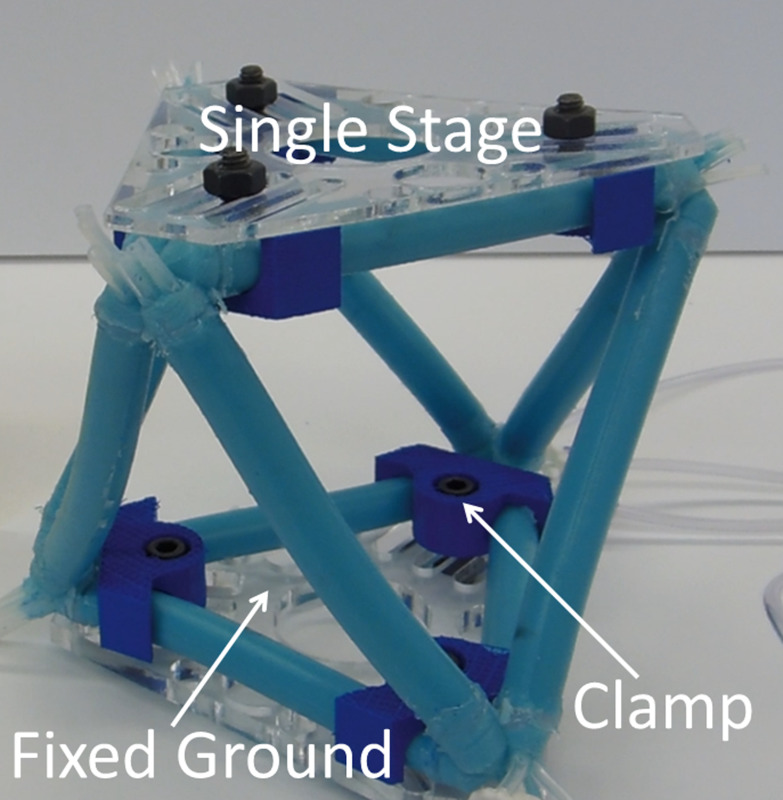
\includegraphics[width=.8\textwidth]{../Notes/figures/soft_parallel.jpg} 
			\end{tcolorbox} 
		\end{column}	
	\end{columns}
	\centering \footnotesize{A soft 6-6 Stewart manipulator. Jonathan Hopkins, 2015.}
\end{frame}



\section{Mobility}

\begin{frame}
	\frametitle{Outline}
	\begin{tcolorbox}[coltitle=yellow!50!black,colframe=magenta!25,split=.2,title=Freedom and Structure]
		Freedoms, Constraints, and Mobility.
		\tcblower
		Motion of linkages: Screws, and spatial motions.
		\vspace{.2cm}
		\newline
		Freedom and Mobility: Freedoms, unfreedoms, connectivity, mobility;
		\vspace{.2cm}
		\newline
		Gr{\"u}bler-Kutzbach's mobility criterion and examples.
	\end{tcolorbox}
\end{frame}
 


\begin{frame}
	\frametitle{Degrees of Freedom and Structure}
	%		
	\begin{definition}[Connection Degree]
		For any  \textcolor{blue}{manipulator joint}, we shall mean its \textcolor{red}{connection degree} to be the \textcolor{red}{number of links attached it}.
	\end{definition}
	%	
	\begin{block}{Quiz}
		What is the connection degree of the u-joints of a Stewart-Gough platform.
	\end{block}
\end{frame}

	\begin{frame}
	\frametitle{Members and Dual Graphs}			
	%
	\begin{tcolorbox}[colframe=blue!80!green, title=Dual graph of a Stewart platform, coltitle=white!80,toggle enlargement=none]
		\begin{columns}[b]
			\begin{column}{\linewidth}			
				\begin{figure}
					\centering 
					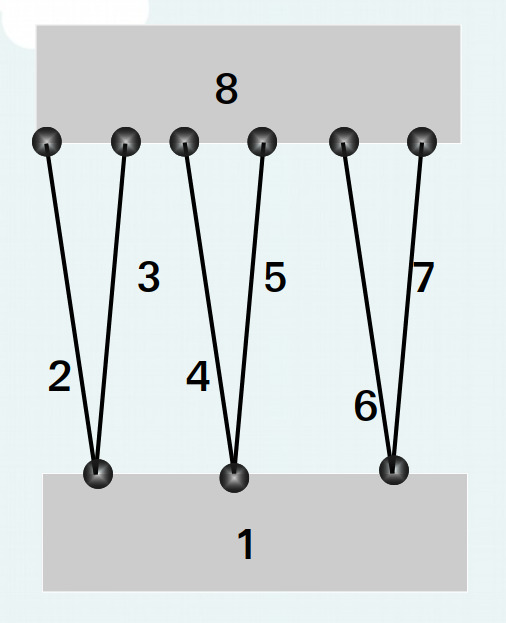
\includegraphics[width=.5\textwidth]{figures/dualgraph_stewart.jpg}
				\end{figure}
			\end{column}	
		\end{columns}
	\end{tcolorbox}
\label{fig:dualgraph}
\end{frame}

\begin{frame}
	\frametitle{Degrees of Freedom and Structure}
	%
	\begin{block}{Members and Freedoms}
		\textcolor{blue}{Degrees of freedoms (or freedoms)} concerns the \textcolor{red}{relative motion of members of a pair} that do not touch one another directly. 
	\end{block}
	%
	\begin{block}{Connectivity}
		By the dual graph of the Stewart platform as seen on Frame \autoref{fig:dualgraph}, the total number of freedoms that \textcolor{red}{connect the two members} (1 and 8) that do not connect to one another directly is \textcolor{blue}{six}. 
	\end{block}
\end{frame}


\begin{frame}
	\frametitle{Planar Linkages}	
	\begin{block}{Four Bar Linkages}
		\begin{columns}[b]
			\begin{column}{\linewidth}		
				\centering 
				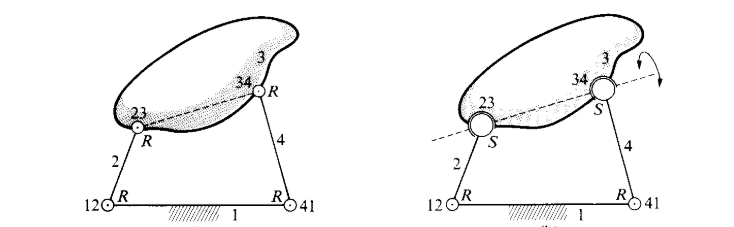
\includegraphics[width=\textwidth]{../Notes/figures/four-bar-linkage.png}
			\end{column}	
		\end{columns}
		\note{The planar $RRRR$ linkage, (\textit{left}) is modified in (\textit{right}) to an $RSSR$ linkage to allow spatial spin-movement of the coupler 3; the connectivity $\mathscr{C}_{13}=2$.}
		\footnotesize{Reprinted from Hunt, 1977: Kinematic Geometry of Mechanisms.}
	\end{block}
	\label{fig:4bar_hunt}
\end{frame}

\begin{frame}
	\frametitle{Freedom from Connectivity}			
	%
	\begin{tcolorbox}[colframe=blue!80!green, title=A (Hacked) Four-Bar Linkage, coltitle=white!80,toggle enlargement=none]
		\begin{columns}[b]
			\begin{column}{.45\linewidth}			
				\begin{figure}
					\centering 
					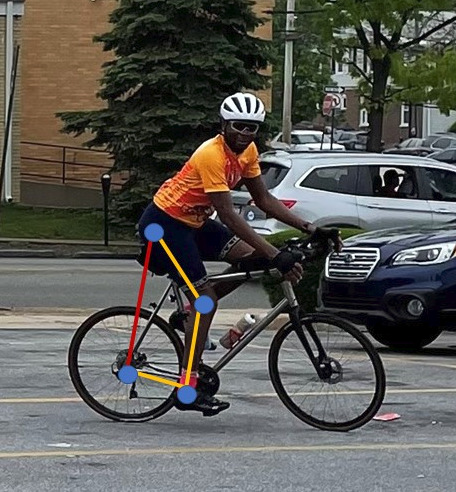
\includegraphics[width=\textwidth]{figures/4bar_me.jpg}
				\end{figure}
			\end{column}
		\begin{column}{.45\linewidth}			
			\begin{figure}
			\centering 
			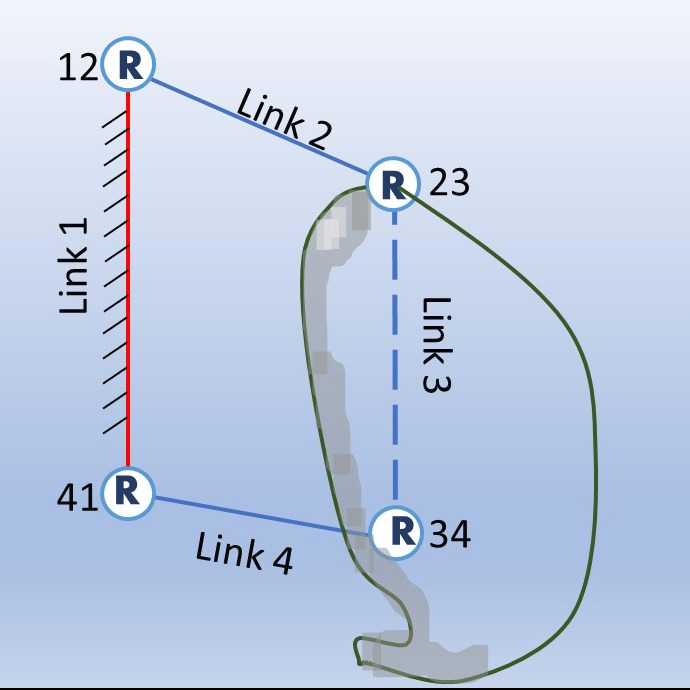
\includegraphics[width=\textwidth]{figures/4bardual.jpg}
			\end{figure}
		\end{column}	
		\end{columns}
	\end{tcolorbox}
	\label{fig:4bar}
\end{frame}


\begin{frame}
	\frametitle{The Four Bar Linkage}
	%
	\begin{block}{Couplings and Freedom}
		
		Links $2 \& 4$ complete a \textcolor{cyan}{coupling or connection} between links $1 \& 3$. 
	\end{block}
	%
	\begin{block}{Connectivity}
		The $R$-pairs are said to have a \textcolor{magenta}{connectivity} of  $\mathscr{C}_{ij}=1$ for all $i,j=1,2,3,4$. Thus, total degree of freedom is $1$.
	\end{block}
\end{frame}

\begin{frame}
	\frametitle{Mobility of Mechanisms}
	%
	\begin{block}{The Mobility and Relative Mobility, $\mathfrak{M}$}
		Simply put, the number of a mechanism's freedoms is its \textcolor{cyan}{mobility}, or \textcolor{cyan}{relative mobility},  $\mathfrak{M}$.  
	\end{block}
	%
	\begin{block}{The Mobility, $\mathfrak{M}$}
		It specifies the \textcolor{green}{independent variables} needed to \textcolor{pink}{determine every relative location} of a \textcolor{red}{mechanism's members}  with respect to one another.
	\end{block}
	%
	\begin{block}{A Note on Serial and Parallel Mobility}
		A little tricky to determine for parallel mechanisms but straightforward for serial mechanisms.
	\end{block}
\end{frame}

\begin{frame}
	\frametitle{Mobility of Mechanisms}
	%
	\begin{block}{Quiz}
		What is the mobility $\mathfrak{M}$ of the $RSSR$ four bar linkage of Frame \ref{fig:4bar_hunt}? Why?
	\end{block}
	%
	\begin{block}{Quiz}
		What is the mobility $\mathfrak{M}$ of the $RRRR$ four bar linkage of Frame \ref{fig:4bar}? Why?
	\end{block}
	%
	\begin{definition}[The mobility criterion (well, not yet)]
		Let's not get ahead of ourselves. A little introduction to screws are in order for us to grasp the \textcolor{red}{Gr{\"u}bler-Kutzbach} mobility criterion.
	\end{definition}
\end{frame}


\subsection{Screws}
\begin{frame}
	\frametitle{Unique Location of a Rigid Body in 3D Space}
	%
	\begin{tcolorbox}[top=0mm, title=Inhomogeneity of Displacements and Angles]
		Quiz: Three translations and three rotations are ill-posed for uniquely determining the freedoms of a body. Why?
		\tcblower
		They are \textcolor{green}{not homogeneous}. 
		\begin{description}
			\item For true \textcolor{blue}{kinematic wholeness and generality}, displacement that is \textcolor{red}{purely translatory} and \textcolor{red}{purely rotary} is needed.
		\end{description}
	\end{tcolorbox}
\end{frame}

\begin{frame}
	\frametitle{Screws for Kinematic Generality}
	%
	\begin{block}{Need for Screws}
		From a kinematic standpoint, \textcolor{red}{six homogeneous screw coordinates} -- each having an \textcolor{cyan}{independent screw freedom} -- are needed to \textcolor{red}{uniquely determine a rigid body's location}.
	\end{block}
	%
	\begin{columns}[b]
		\begin{column}{.7\columnwidth}
			\begin{definition}[What is a screw anyway?]
				A \textcolor{blue}{screw} is a \textcolor{red}{straight line} in space, called \textcolor{blue}{the axis}, with an associated direction, called \textcolor{blue}{pitch}, $p$.
			\end{definition}
		\end{column}
		\begin{column}{.25\columnwidth}
			\centering
			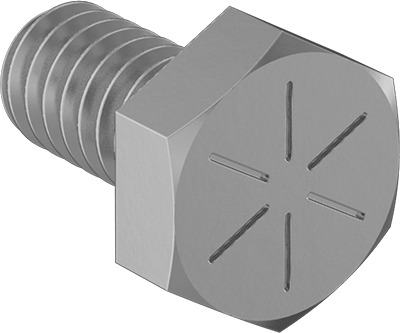
\includegraphics[width=\textwidth]{figures/screw.jpg}
		\end{column}
	\end{columns}
\end{frame}

\begin{frame}
	\frametitle{Unique Location of a Rigid Body in 3D Space}
	%
	\begin{columns}[b]
		\begin{column}{.65\columnwidth}
			\begin{definition}[Screw Coordinates]
				Six-vector, $\bm{s}$, related to the Pl{\"u}cker coordinates (see right inset) parameterize a screw i.e. $\bm{s}=\left(s_1, s_2, s_3, s_4, s_5, s_6\right)$.
			\end{definition}
		\end{column}
		\begin{column}{.3\columnwidth}
			\centering
			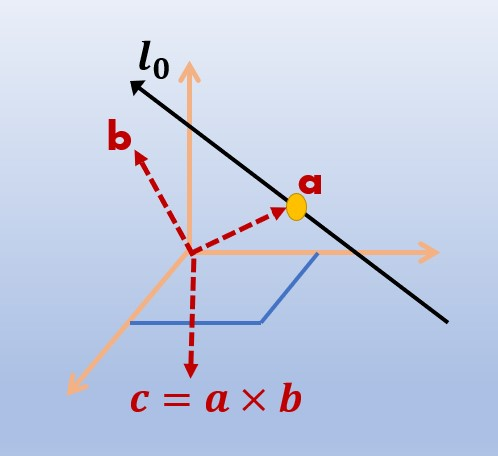
\includegraphics[width=\textwidth]{figures/plucker_coords.jpg}
		\end{column}
		\label{fig:plucker}
	\end{columns}
	%
	\begin{block}{Pl{\"u}cker Coordinates}
		Let \textcolor{red}{$\bm{a}$} be a point on line $\bm{\ell}_0$. Let \textcolor{red}{$\bm{a}$}'s direction cosine vector (to be introduced shortly) be \textcolor{red}{$\bm{b}$}. Then, its binormal (moment) vector is \textcolor{red}{$\bm{c=a\times b}$}. We say the pair \textcolor{red}{$(\bm{b},\bm{c})$} is the \textcolor{blue}{Pl{\"u}cker Coordinates} of the point  \textcolor{red}{$\bm{a}$ on axis $\bm{\ell}_0$}.
	\end{block}
\end{frame}


\subsection{Pl{\"u}cker coordinates}
\begin{frame}
	\frametitle{Screws and Pl{\"u}cker Coordinates Relationship}
	%
	\begin{block}{Screw axis and Pl{\"u}cker Coordinates Relationship}
		\begin{align}
			b_1 &= s_1, \quad b_2 = s_2, \quad b_3 = s_3 \\
			c_1 &= s_4 - ps_1, \quad c_2 = s_5-ps_2, \quad c_3 = s_6 - ps_3.
		\end{align}
	$p$: pitch! How to find it?
	\end{block}
	%
	\begin{block}{Screw and Pl{\"u}cker Coordinates Relationship}
		Suppose that 
		\begin{align}
			h &= \sqrt{b_1^2+b_2^2+b_3^2}.
		\end{align}
		Then $(\bm{b}/h, \bm{c}/h)$ are respectively the direction cosines of the line, $l_0$ and its moment.
	\end{block}
\end{frame}

\begin{frame}
	\frametitle{Pitch and Magnitude of the screw}	
	\begin{block}{Pitch of a screw}
		\begin{align}
			p &= \dfrac{s_1 \, s_4 + s_2 \, s_5 + s_3 \, s_6}{\sqrt{s_1^2 + s_2^2 + s_3^2}}, \\
			\mid s \mid &= \sqrt{s_1^2 + s_2^2 + s_3^2} \quad \text{if } p \neq \infty \\
			\mid s \mid &= \sqrt{s_4^2 + s_5^2 + s_6^2} \quad \text{if } p = \infty
		\end{align}
	\end{block}
\end{frame}
%
\begin{frame}
	\frametitle{Pl{\"u}cker Coordinates Example}
	\begin{block}{Chasles' Theorem Applied to The Serret-Frenet Frame}
		Consider a spatial curve $\bm{C}$ on the elephant continuum trunk shown earlier. Suppose $\bm{C}$ is parameterized by its arc length $\bm{s} \in [0, 1]$. For a point $\bm{x}=\left[x, y, z\right]^T$ on $\bm{C}$, the unit tangent vector to $\bm{C}$ is $\bm{t}=\bm{dx}/\bm{ds}$. Denote by $\bm{n}$ the principal normal to $\bm{C}$ at $\bm{n}$; then we must have $\bm{b}=\bm{t}\times \bm{n}$ as the binormal. We say $(\bm{b},\bm{n})$ together form the Pl{\"u}cker coordinates of the tangent $\bm{t}$.
	\end{block}
	%
	%
	\begin{columns}[]
		\begin{column}{.5\columnwidth}
			\centering
			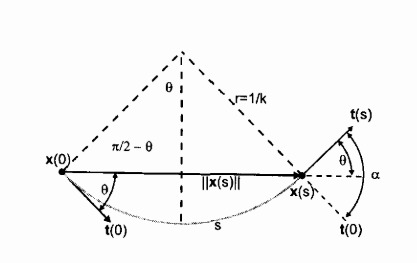
\includegraphics[width=\textwidth]{figures/serret.jpg}
		\end{column}
	\end{columns}
\end{frame}

\begin{frame}
	\frametitle{Pl{\"u}cker Coordinates Example}
	%
	\begin{block}{Poinsot's Theorem Quiz on a  Force and its Moment}
		Suppose that a force $\bm{F}$  acts at the point $\bm{a}$ in the image of Frame \ref{fig:plucker}. What are the Pl{\"u}cker coordinates of the \textcolor{red}{line of force}?
	\end{block}
	%
	\begin{block}{ Homogeneous Coordinates!}
		\textcolor{blue}{Pl{\"u}cker Coordinates} give six unit parameters of a point on a line. Pl{\"u}cker Coordinates are in \textcolor{red}{homogeneous coordinates}!
	\end{block}
\end{frame}

\note{
\begin{frame}
	%
	\begin{block}{Poinsot's Theorem Quiz on a  Force and its Moment}
		Imagine that a force $\bm{F}$ is acting at the point $\bm{a}$ in the image of Frame \ref{fig:plucker}. Suppose that $\bm{\tau}$ is torque acting along the normal to point $\bm{a}$.  Then $(\bm{f,\tau})$ are the Pl{\"u}cker  coordinates of the \textcolor{red}{line of force}.
	\end{block}
	%
	\begin{block}{Arithmetics on Screws}
		Scalar and vector arithmetic operations are valid on infinitesimal  screws e.g.
		\begin{align}
			c_1 \bm{s}_1 + c_2 \bm{s}_2 = 0 \text{ for } c_1, \, c_2 \neq 0 \text{ on screws } \bm{s}_1, \bm{s}_2.
		\end{align}
	\end{block}
\end{frame}
}

\subsection{Freedoms and Constraints}
\begin{frame}
	\frametitle{Freedoms, Unfreedoms, and Mobility}
	%
	\begin{block}{Freedom and Constraints}
		Suppose a screw $\bm{f}=(f_1,\cdots, f_6)$ ``fixes" a body in 3D space. 
		\begin{description}
			\item Each \textcolor{red}{constraint} $u_i \neq f_j$ for $(i,j)\in \{1,\cdots,6\}$.
			%
			\item Rather each \textcolor{red}{$u_i$} has influence on every $\{f_i\}_{i=1}^{6}$.
			%
			\item Each $u_i$ from the six independent equations, $g(s_1, s_2, s_3, s_4, s_5, s_6)=0$, suppresses a \textcolor{cyan}{freedom}, $f_i$.
			%
			\item Progressively relaxing each \textcolor{red}{$u_i$}, \textcolor{red}{or unfreedom}, adds an extra body $f_i$.
		\end{description}
	\end{block}
	%
\end{frame}


\begin{frame}
	\frametitle{Freedoms, Unfreedoms, and Mobility}
	%
	\begin{block}{Freedom and Unfreedoms}
		Suppose the total \textcolor{blue}{freedoms} is $\bm{f}$ and the total \textcolor{red}{unfreedoms} is $\bm{u}$, then
		\begin{description}
			\item $\bm{u}+\bm{f}=6.$
			\label{eq:freedomunfreedom}
		\end{description}
	Note: A rigid body's freedoms is also referred to the dimension of  its \textcolor{blue}{configuration space}.
	\end{block}
	%
	\begin{block}{Relative Freedoms}
		Suppose there are a total of $n$ \textcolor{red}{unconstrained} bodies. Suppose further that we choose one out of the bodies as a reference body. Then the total number of \textcolor{green}{relative freedoms} is $6(n-1)$.
	\end{block}
\end{frame}

\begin{frame}
	\frametitle{Freedoms, Unfreedoms, and Mobility}
	\begin{block}{Constraints and Joints}
		Now, consider $k$ \textcolor{red}{independent constraints}\footnote{NB: The total \textit{allowable} constraints is 5 for a body in relative motion. It is 6 for a fully rigid body.} such as \textcolor{blue}{joints} \textcolor{green}{along points, lines, curves or surfaces}.
	\end{block}
	
	\begin{block}{The Mobility Criterion}
		Let the \textcolor{red}{constraint} of joint, $i$ (e.g. a joint along points, lines, curves or surfaces) be $u_i$. Then the mobility criterion $\mathfrak{M}$ is
		\begin{align}
			\mathfrak{M}=6(n-1) - \sum_{i=1}^{k}u_i.
		\end{align}
	\end{block}
\end{frame}

\subsection{Mobility Criterion}

\subsection{Mobility Criterion}
\begin{frame}
	\frametitle{ General Gr{\"u}bler-Kutzbach Mobility Criterion}	
	\begin{block}{ General Gr{\"u}bler-Kutzbach Mobility Criterion}
		Recall that $\sum_i u_i + f_i = 6$ from Frame \eqref{eq:freedomunfreedom} so that 
		\begin{align}
			\mathfrak{M}=6(n-k-1) - \sum_{i=1}^{f}f_i.
			\label{grubler}
		\end{align}
	\end{block}
	
	\begin{block}{Exceptions: Relative Planar and Spherical Motions}
		For bodies restricted to relative planar or spherical  motions, the total freedoms + constraints is 3 (not 6)! %Therefore, 
		\begin{align}
			\mathfrak{M}=3(n-k-1) - \sum_{i=1}^{f}f_i.
			\label{grubler}
		\end{align}
	\end{block}
\end{frame}

\begin{frame}
	\frametitle{ General Gr{\"u}bler-Kutzbach Criterion References}
		
	\begin{block}{The Gr{\"u}bler-Kutzbach Mobility Criterion References}
		Attributed to Gr{\"u}bler: 
		\begin{description}
			\item \footnotesize{Schoenflies, Arthur, and M. Grübler. ``Kinematik." In Encyklopädie der Mathematischen Wissenschaften mit Einschluss ihrer Anwendungen, pp. 190-278. Vieweg+Teubner Verlag, Wiesbaden, 1908};
			\item \footnotesize{Grübler, Martin Fürchtegott. Getriebelehre: eine Theorie des Zwanglaufes und der ebenen Mechanismen. Springer, 1917}.
		\end{description}
	and Kutzbach:
		\begin{description}
			\item \footnotesize{Kutzbach, Karl. "Mechanische leitungsverzweigung, ihre gesetze und anwendungen." Maschinenbau 8, no. 21 (1929): 710-716.}
		\end{description}
	\end{block}
\end{frame}

\begin{frame}
	\frametitle{Loops}	
	\begin{block}{Loops}
		A \textcolor{blue}{kinematic chain} often comprises \textcolor{blue}{members} called \textcolor{green}{loops}. 
	\end{block}
	
	\begin{block}{Binary Link}
		Members in a \textcolor{blue}{binary link} constitute a \textcolor{green}{single loop}. Example: The four-bar linkage. 
	\end{block}	
	
	\begin{block}{Single loops}
		For \textcolor{blue}{single loops}, $k=n$ so that $\mathfrak{M}=\sum_{i=1}^{f} f_i - 6$. 
	\end{block}
	
	\begin{block}{Mobility of Mechanisms}
		$\mathfrak{M}\le 1$ for at least one actuator-pair to produce mobility at a successor joint which depends on that actuator-pair's input. 
	\end{block}
\end{frame}


%
\begin{frame}
	\frametitle{Mobility of Common Robot Configurations}
	%
	\begin{columns}[]
		%
		\begin{column}{.5\linewidth}
			\centering
			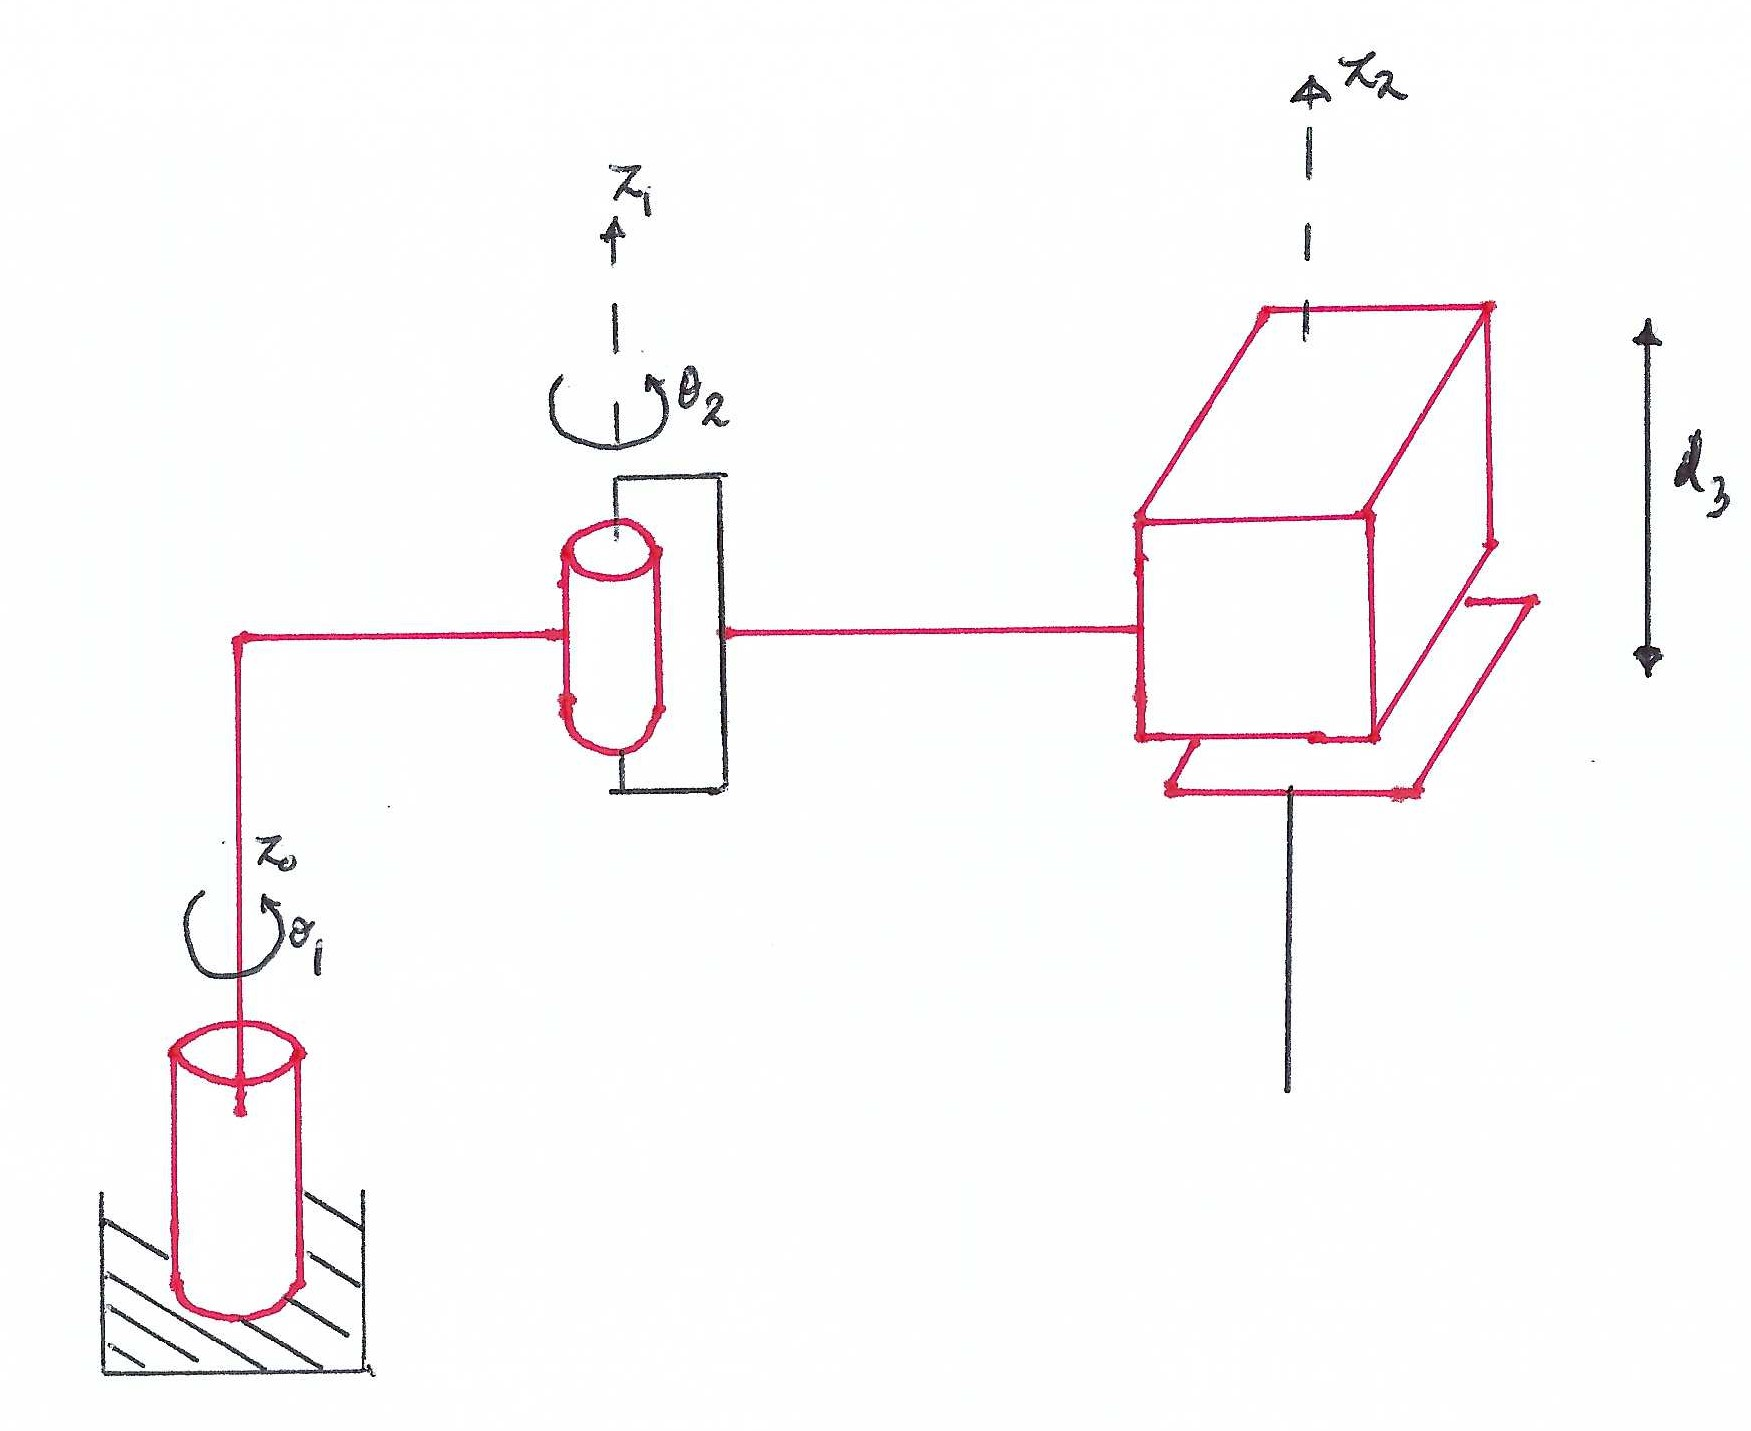
\includegraphics[width=\textwidth]{figures/scara_schematic.jpg}
			\footnotesize{Configuration of the SCARA Arm.}
		\end{column}
		%
		\begin{column}{.5\linewidth}
			\centering
			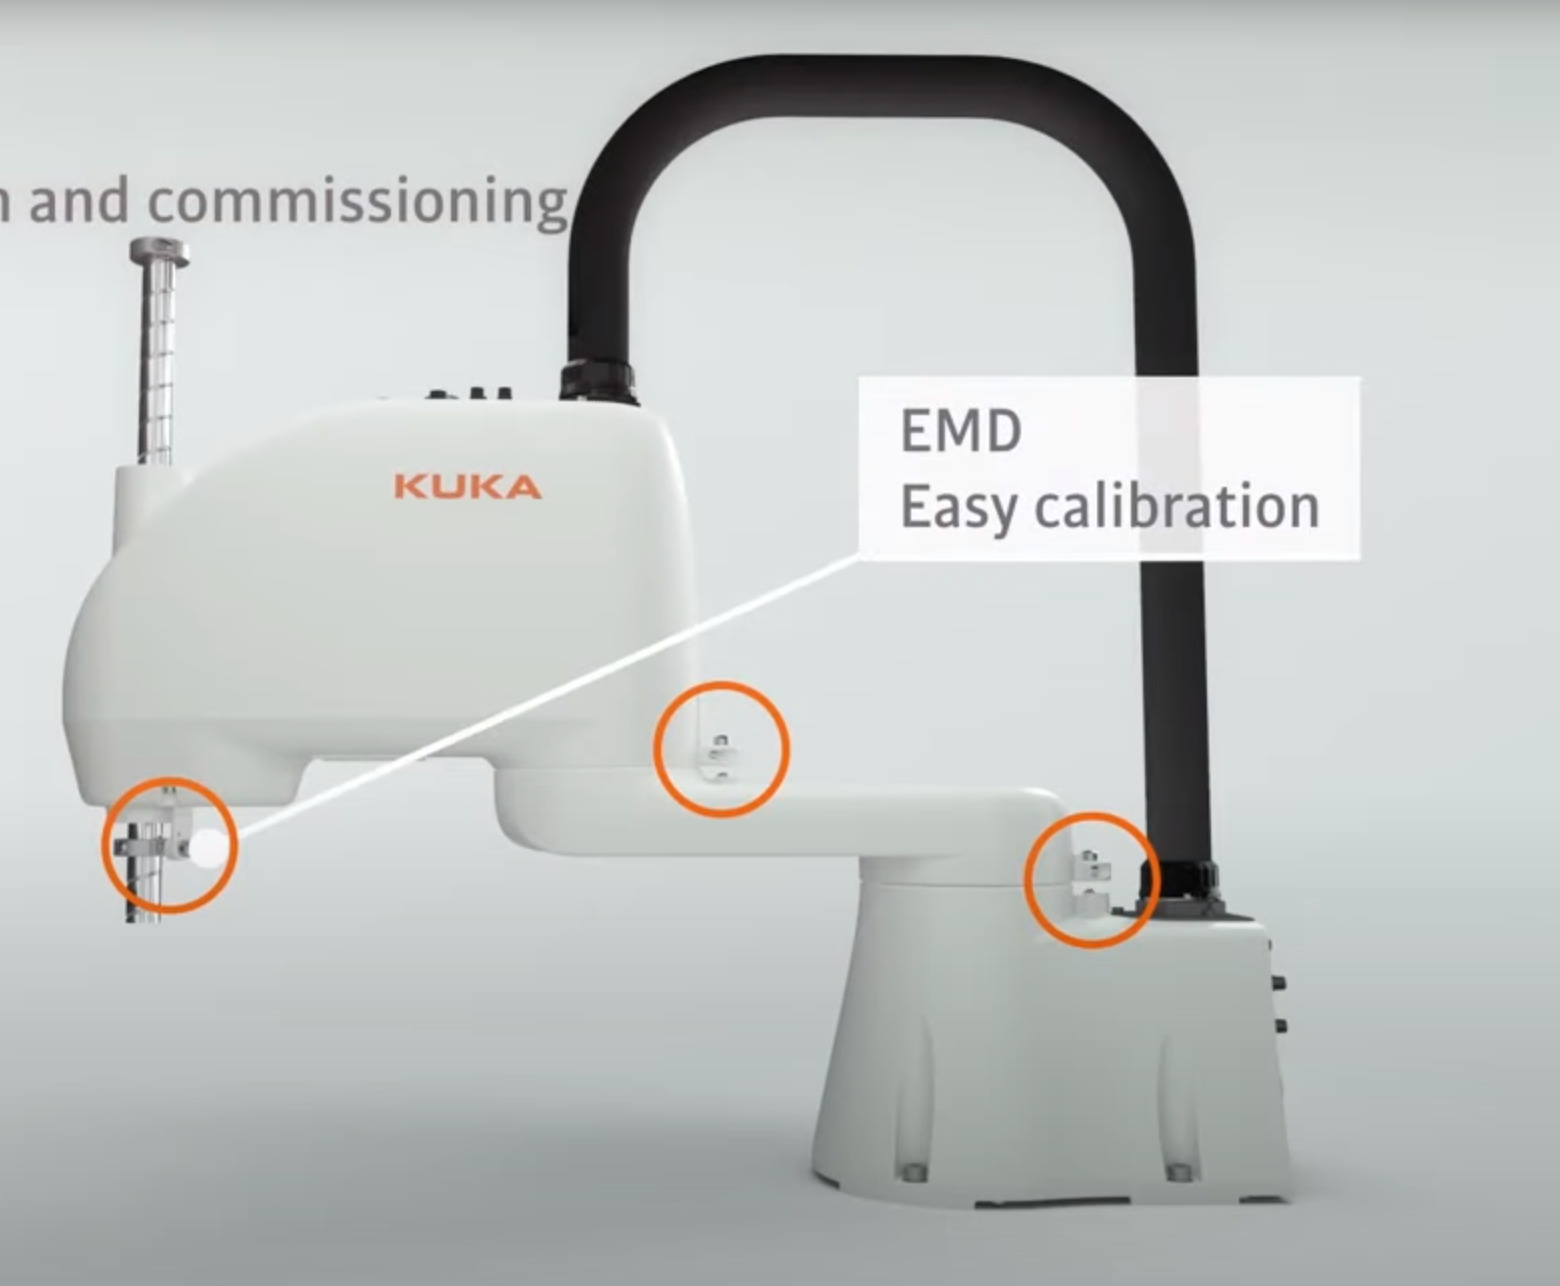
\includegraphics[width=\textwidth, rotate=360]{figures/Scara.jpg}
			\footnotesize{Courtesy of Fanuc America Inc.}
		\end{column}
	\end{columns}
\end{frame}
%
\begin{frame}
	\frametitle{Mobility of The SCARA Robot}
	%
	\begin{columns}[]
		%
		\begin{column}{.5\linewidth}
			\begin{block}{Mobility Analysis}
				Two rotary joints. One prismatic joint acting along the $z$ axis, and constrained along the $xy$ plane. 
			\end{block}
		\end{column}
	%
		\begin{column}{.5\linewidth}
			\begin{block}{Mobility Parameters}			
			Four rigid bodies (links). Three constraints.  Four freedoms. Therefore, $\mathfrak{M}=6(4-3-1)+4=4$
			\end{block}
		\end{column}
	\end{columns}
\end{frame}

\begin{frame}
	\frametitle{Mobility Analysis of The Universal Robot}
	%
	\begin{columns}[]
		%
		\begin{column}{.5\linewidth}
			\centering
			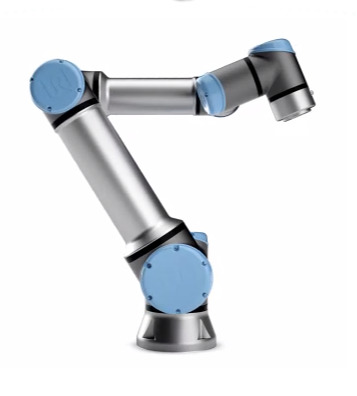
\includegraphics[width=\textwidth]{figures/ur16.jpg}
			\footnotesize{\copyright Universal Robots A/S, DK.}
		\end{column}
		%
		\begin{column}{.5\linewidth}
			\centering
			\begin{block}{The Revolute Arm}
				\footnotesize{Falls under so-called $RRR$ kinematic arrangements. Also called a \textcolor{blue}{revolute}, \textcolor{blue}{elbow}, or \textcolor{blue}{anthorpomorphic manipulator}.}
			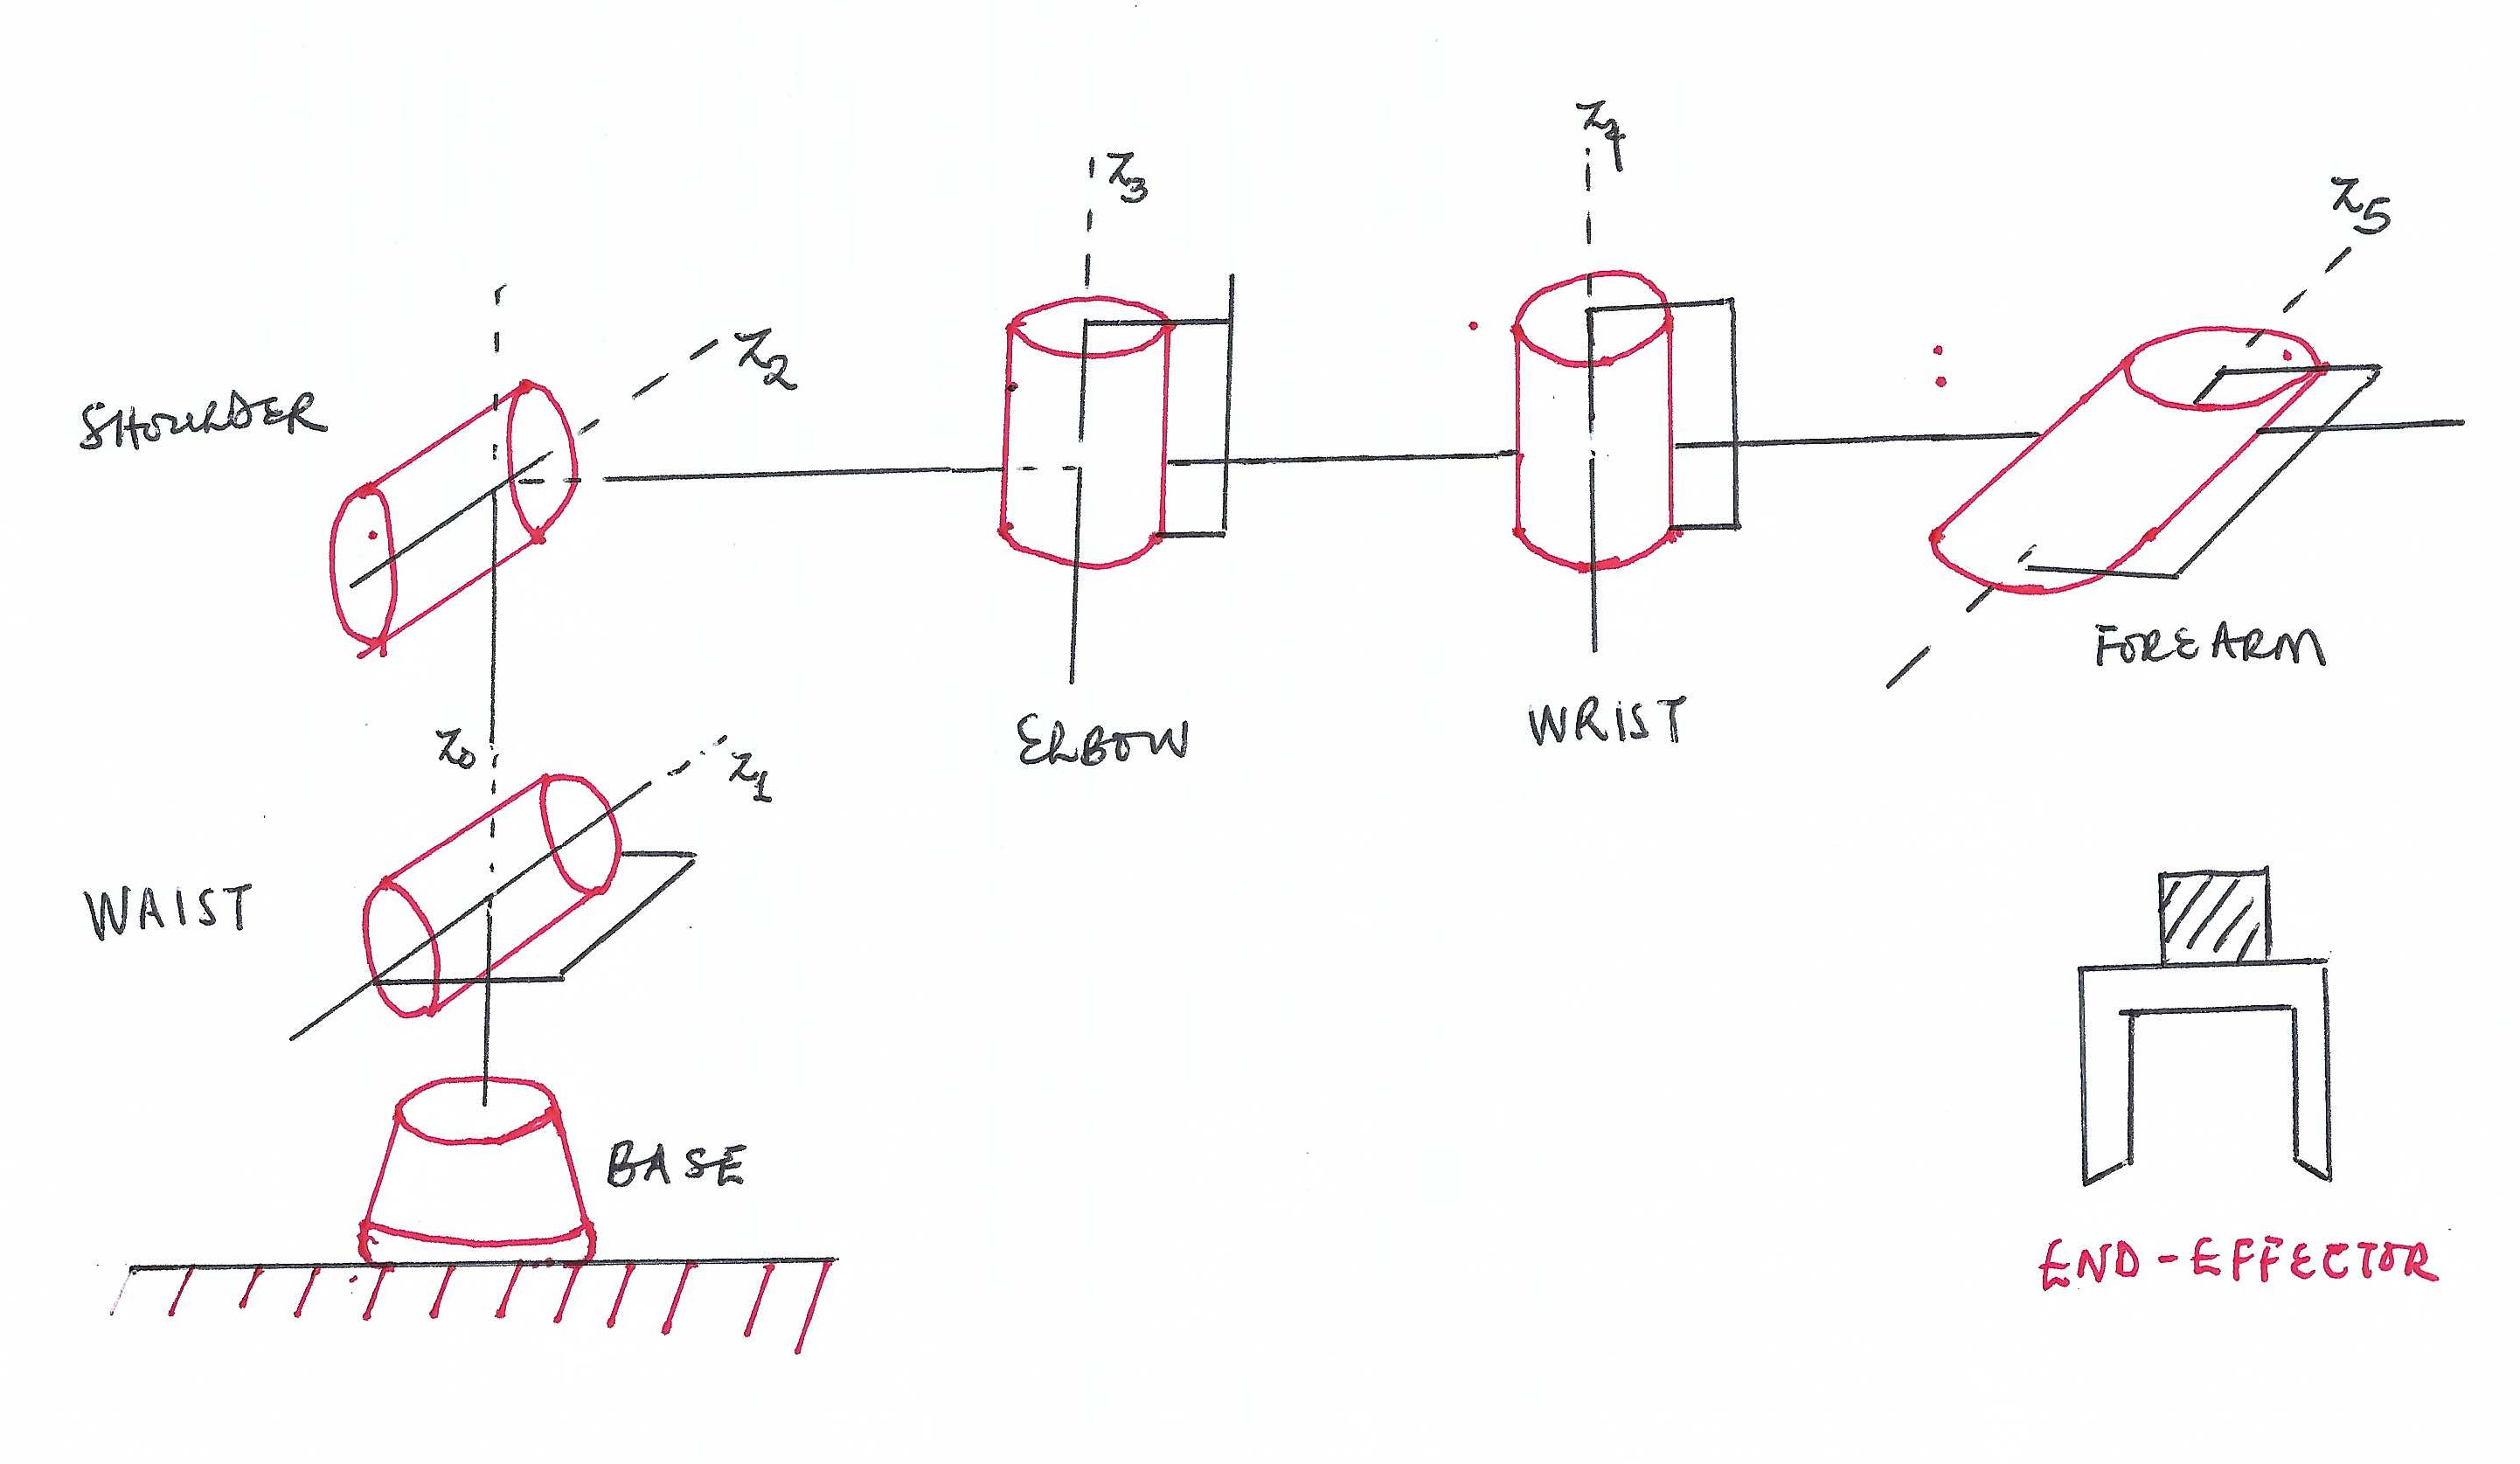
\includegraphics[width=\textwidth]{figures/ur_scheme.jpg}
			$n=6; \, k=6; \, f=5\times3:=18$ $\therefore \mathfrak{M}=6(n-k-1)+\sum f_i $ $\implies 6(6-1-5) + 18$ or $\mathfrak{M}=6$.
			\end{block}
		\end{column}
	\end{columns}
\end{frame}

\begin{frame}
	\frametitle{Mobility of The Stewart-Gough Platform}
	%	
	\centering 
	\begin{columns}
		\begin{column}{.4\linewidth}
			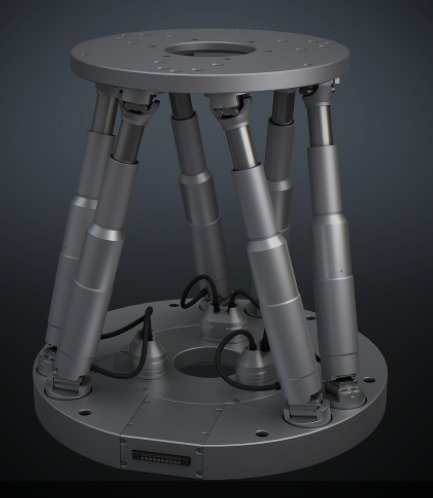
\includegraphics[width=\textwidth]{figures/stewart_spherical.jpg}
		\end{column}
		%\begin{columns}
		\begin{column}{.25\linewidth}
			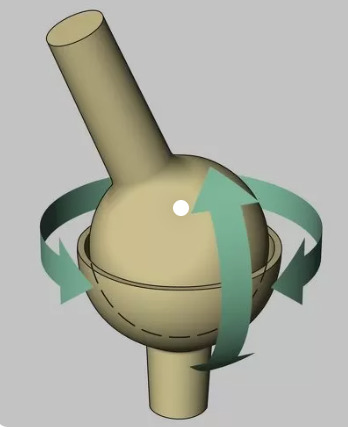
\includegraphics[width=\textwidth]{figures/spherical.jpg}
			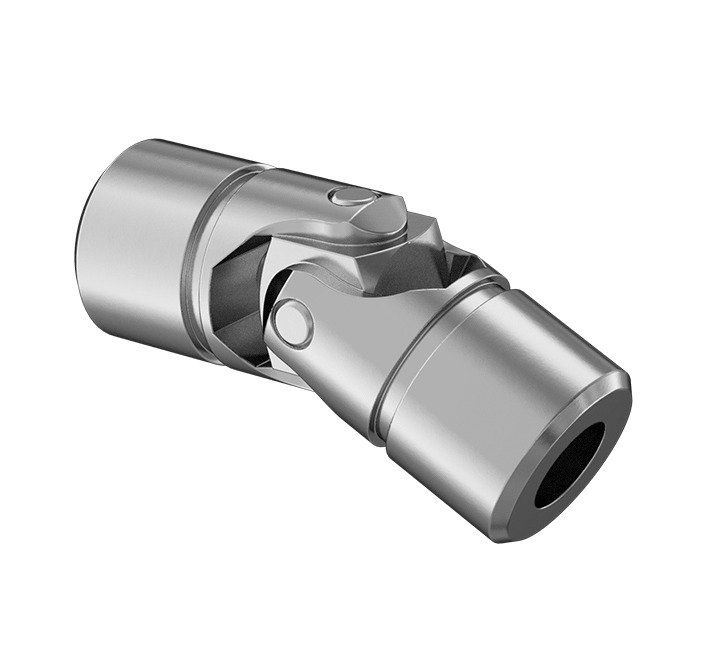
\includegraphics[width=\textwidth]{figures/ujoint.jpg}	
		\end{column}
		%\end{columns}
	\end{columns}	
\end{frame}

\begin{frame}
	\frametitle{Mobility of The Stewart-Gough Platform}
	%
	\begin{columns}[]
		%
		\begin{column}{.45\linewidth}
			\begin{block}{Unconstrained bodies, $n$}
				There are \textcolor{blue}{six universal joints} that connect \textcolor{blue}{the base platform} to the prismatic linear actuators. There are \textcolor{blue}{six spherical joints} that connect \textcolor{blue}{the top platform} to the top of the prismatic actuators. Altogether, there are $n=6+6+2$ or $14$ unconstrained \textcolor{red}{rigid links}.
			\end{block}
		\end{column}
		%
		\begin{column}{.55\linewidth}
			\begin{block}{Constraints, $k$}			
				Six \textcolor{blue}{u-joints}. Six \textcolor{blue}{spherical joints}.  Six \textcolor{blue}{prismatic joints}. Altogether, there are $f=6+6+6:=18$ \textcolor{blue}{constraints}.
			\end{block}
			\begin{block}{Freedoms, $f$}			
				Each \textcolor{blue}{u-joints has two freedoms}. Each \textcolor{blue}{spherical joint has three (rotary) freedoms}.  Each \textcolor{blue}{prismatic joint has one freedom}. Altogether, there are $f=6\times2+6\times3+6\times1:=36$ \textcolor{blue}{freedoms}.
			\end{block}
		
		\end{column}
	\end{columns}
\end{frame}


% ---- Bibliography ----
\bibliographystyle{../../Proposal/styles/bibtex/spmpsci_unsrt}
{
\tiny
\bibliography{../../../SRS/Continuum/biblio}
}
\end{document}
